\documentclass{article}
\usepackage[margin=1in]{geometry}
\usepackage{amsmath,amsthm,amssymb,mathrsfs}
\usepackage{graphicx}
\usepackage[pdfencoding=auto, psdextra]{hyperref}
\usepackage[figurename=Figure]{caption}
\usepackage{booktabs}
\usepackage{enumitem}
\usepackage{tikz,tikz-cd}
\usetikzlibrary{positioning, arrows.meta}
\usepackage{algorithm}
\usepackage{algpseudocode}
\usepackage{xcolor}

\newtheorem{theorem}{Theorem}
\newtheorem{lemma}{Lemma}
\newtheorem{prop}{Proposition}
\newtheorem{remark}{Remark}
\newtheorem{conjecture}{Conjecture}
\newtheorem{definition}{Definition}

\newcommand{\mathpdf}[2]{\texorpdfstring{$#1$}{#2}}

\title{Sprecher Networks: A Parameter-Efficient Architecture \\ Inspired by the Kolmogorov--Arnold--Sprecher Theorem}
\author{
  Christian Hägg\thanks{Department of Mathematics, Stockholm University, Stockholm, Sweden. Email: \texttt{hagg@math.su.se}} \and
  Kathlén Kohn\thanks{Department of Mathematics, KTH Royal Institute of Technology, Stockholm, Sweden. Email: \texttt{kathlen@kth.se}} \and
  Giovanni Luca Marchetti\thanks{Department of Mathematics, KTH Royal Institute of Technology, Stockholm, Sweden. Email: \texttt{glma@kth.se}} \and
  Boris Shapiro\thanks{Department of Mathematics, Stockholm University, Stockholm, Sweden. Email: \texttt{shapiro@math.su.se}}
}
\date{\today}

\begin{document}

\maketitle

\begin{abstract}
We present \emph{Sprecher Networks} (SNs), a family of trainable neural architectures inspired by the classical Kolmogorov--Arnold--Sprecher (KAS) construction for approximating multivariate continuous functions. Distinct from Multi-Layer Perceptrons (MLPs) with fixed node activations and Kolmogorov-Arnold Networks (KANs) featuring learnable edge activations, SNs utilize shared, learnable splines (\emph{monotonic} and \emph{general}) within structured blocks incorporating explicit learnable shifts and mixing weights. Our approach directly realizes Sprecher's specific 1965 ``sum of shifted splines'' formula in its single-layer variant and extends it to deeper, multi-layer compositions. Additionally, we introduce a novel soft routing mechanism for residual connections that maintains parameter efficiency while learning adaptive, differentiable connection patterns between layers of different dimensions. We demonstrate empirically that composing these blocks into deep networks leads to highly parameter-efficient models, discuss theoretical motivations, and compare SNs with related architectures (MLPs, KANs, and networks with learnable node activations).
\end{abstract}

\section{Introduction and historical background}
Approximation of continuous functions by sums of univariate functions has been a recurring theme in mathematical analysis and neural networks. The Kolmogorov--Arnold Representation Theorem \cite{kolmogorov, arnold} established that any multivariate continuous function $f : [0,1]^d \to \mathbb{R}$ can be represented as a finite composition of continuous functions of a single variable and the addition operation. Specifically, Kolmogorov (1957) showed that such functions can be represented as a finite sum involving univariate functions applied to sums of other univariate functions of the inputs.

\vspace{1mm}
\textbf{David Sprecher's 1965 construction.} In his 1965 landmark paper \cite{sprecher1965}, David Sprecher provided a constructive proof and a specific formula realizing the Kolmogorov--Arnold representation. He showed that any continuous function $f:[0,1]^n \to \mathbb{R}$ could be represented as:
\begin{equation}\label{eq:sprecher_original}
f(\mathbf{x})=\sum_{q=0}^{2n}\Phi\Biggl(\,\sum_{p=1}^{n}\lambda_p\,\phi\bigl(x_p+\eta\,q\bigr)+q\Biggr)
\end{equation}
for a single \emph{monotonic} inner function $\phi$, a continuous outer function $\Phi$, a constant shift parameter $\eta > 0$, and constants $\lambda_p$. This construction simplified the representation by using only one inner function $\phi$, relying on shifts of the input coordinates ($x_p + \eta q$) and an outer summation index shift ($+q$) to achieve universality. The key insight of \emph{shifting input coordinates} and summing evaluations under inner and outer univariate maps is central to Sprecher's specific result.

\vspace{1mm}
\textbf{From a shallow theorem to a deep architecture.} Sprecher's 1965 result is remarkable because it guarantees universal approximation with a single hidden layer (i.e., a shallow network). This mirrors the history of Multi-Layer Perceptrons, where the Universal Approximation Theorem also guaranteed the sufficiency of a single hidden layer. However, the entire deep learning revolution was built on the empirical discovery that composing multiple layers, while not theoretically necessary for universality, provides vast practical benefits in terms of efficiency and learnability.

This history motivates our central research question: can the components of Sprecher's shallow, highly-structured formula be used as a new kind of building block in a \emph{deep}, compositional architecture? We propose to investigate this by composing what we term \emph{Sprecher blocks}, where the vector output of one block becomes the input to the next. It is crucial to emphasize that this deep, compositional structure is our own architectural proposal, inspired by the paradigm of deep learning, and is not part of Sprecher's original construction or proof of universality. The goal of this paper is not to generalize Sprecher's theorem, but to empirically evaluate whether this theorem-inspired design is a viable and efficient alternative to existing deep learning models when extended into a deep framework.

\vspace{1mm}
\textbf{Modern context.} Recent work has revitalized interest in leveraging Kolmogorov-Arnold representations for modern deep learning. Notably, Kolmogorov-Arnold Networks (KANs) \cite{liu2024kan} were introduced, proposing an architecture with learnable activation functions (splines) placed on the \emph{edges} of the network graph, replacing traditional linear weights and fixed node activations.

\vspace{1mm}
\textbf{Architectural landscape.} Understanding how novel architectures relate to established ones is crucial. Standard Multi-Layer Perceptrons (MLPs) \cite{haykin1994neural} employ fixed nonlinear activation functions at nodes and learnable linear weights on edges, justified by the Universal Approximation Theorem \cite{cybenko1989approximation, hornik1989multilayer}. Extensions include networks with \emph{learnable activations on nodes}, sometimes called Adaptive-MLPs or Learnable Activation Networks (LANs) \cite{goyal2019learning, zhang2022neural, liu2024kan} (Appendix B), which retain linear edge weights but make the node non-linearity trainable. KANs \cite{liu2024kan} represent a more significant departure, moving learnable splines to edges and eliminating linear weights entirely, using simple summation at nodes. Sprecher Networks (SNs), as we detail below, propose a distinct approach derived directly from Sprecher's 1965 formula. SNs employ function blocks containing shared learnable splines ($\phi, \Phi$), learnable mixing weights ($\lambda$), and explicit structural shifts ($\eta, q$). A key innovation in our approach is the use of \emph{soft routing} for residual connections when dimensions mismatch. Rather than using expensive matrix projections ($O(N^2)$ parameters) or fixed patterns, SNs employ learnable soft assignments with only $O(N)$ parameters, discovering optimal routing patterns through gradient descent. This maintains parameter efficiency while providing the flexibility needed for effective optimization. This structure offers a different alternative within the landscape of function approximation networks.

\section{Motivation and overview of Sprecher Networks}
While MLPs are the workhorse of deep learning, architectures inspired by KAS representations offer potential benefits, particularly in interpretability and potentially parameter efficiency for certain function classes. KANs explore one direction by placing learnable functions on edges. Our \emph{Sprecher Networks} (SNs) explore a different direction, aiming to directly implement Sprecher's constructive formula within a trainable framework and extend it to deeper architectures.

SNs are built upon the following principles, directly reflecting Sprecher's formula:
\begin{itemize}
    \item Each functional block (mapping between layers) is organized around a shared \emph{monotonic} spline $\phi(\cdot)$ and a shared \emph{general} spline $\Phi(\cdot)$, both learnable.
    \item Each block incorporates a learnable scalar shift $\eta$ applied to inputs based on the output index $q$.
    \item Each block includes learnable mixing weights $\lambda_{i}$ (a vector, not a matrix) that combine contributions from different input dimensions, with the same weights shared across all output dimensions.
    \item The structure explicitly includes the additive shift $q$ inside the outer spline $\Phi$, mimicking Sprecher's formulation.
\end{itemize}
Our architecture generalizes this classical single-layer shift-and-sum construction to a multi-layer network by composing these functional units, which we term \emph{Sprecher blocks}. The mapping from one hidden layer representation to the next is realized by such a block. Unlike MLPs with fixed node activations, LANs with learnable node activations, or KANs with learnable edge activations, SNs concentrate their learnable non-linearity into the two shared splines per block, applied in a specific structure involving shifts and learnable linear weights. This imposes a strong inductive bias, trading the flexibility of independent weights/splines for extreme parameter sharing. Diversity in the transformation arises from the mixing weights ($\lambda$) and the index-dependent shifts ($q$).

Concretely, each Sprecher block applies the transformation:
$$ (x_i)_{i=1}^{d_{\mathrm{in}}} \;\mapsto\; \Bigl[\Phi\Bigl(\sum_{i=1}^{d_{\mathrm{in}}}\lambda_{i}\,\phi(x_i+\eta\,q)+q\Bigr)\Bigr]_{q=0}^{d_{\mathrm{out}}-1}.$$
Note that $\lambda_i$ depends only on the input index $i$, not on the output index $q$, maintaining fidelity to Sprecher's original 1965 construction.
For scalar outputs, the outputs of the final Sprecher block are aggregated (via summation over $q$). For vector outputs, an additional block is used without final summation.

In Sprecher's original work, one layer (block) with $d_{\mathrm{out}} = 2n+1$ outputs (where $n=d_{\mathrm{in}}$) was sufficient for universality. Our approach stacks $L$ Sprecher blocks to create a deep network progression:
$$ d_0 \to d_1 \to \cdots \to d_{L-1} \to d_L, $$
where $d_0=d_{\mathrm{in}}$ is the input dimension, and $d_L$ is the dimension of the final hidden representation before potential aggregation or final mapping. This multi-block composition provides a deeper analog of the KAS construction, aiming for potentially enhanced expressive power or efficiency for complex compositional functions. The universality of networks with \(L>1\) blocks or vector-valued outputs is an open question we explore empirically (see Section~\ref{sec:universality}).

\begin{definition}[Network notation]
Throughout this paper, we denote Sprecher Network architectures using arrow notation of the form $d_{\mathrm{in}}\to[d_1,d_2,\ldots,d_L]\to d_{\mathrm{out}}$, where $d_{\mathrm{in}}$ is the input dimension, $[d_1,d_2,\ldots,d_L]$ represents the hidden layer dimensions (widths), and $d_{\mathrm{out}}$ is the final output dimension of the network. For scalar output ($d_{\mathrm{out}}=1$), the final block's outputs are summed. For vector output ($d_{\mathrm{out}}>1$), an additional non-summed block maps from $d_L$ to $d_{\mathrm{out}}$. For example, $2\to[5,3,8]\to1$ describes a network with 2-dimensional input, three hidden layers of widths 5, 3, and 8 respectively, and a scalar output (implying the final block's outputs of dimension 8 are summed). $2\to[5,3]\to4$ describes a network with 2-dimensional input, two hidden layers of widths 5 and 3, and a 4-dimensional vector output (implying an additional output block maps from dimension 3 to 4 without summation). When input or output dimensions are clear from context, we may use the abbreviated notation $[d_1,d_2,\ldots,d_L]$ to focus on the hidden layer structure.
\end{definition}

\section{Core architectural details}
In our architecture, the fundamental building unit is the \emph{Sprecher block}. The network is composed of a sequence of Sprecher blocks, each performing a shift-and-sum transformation inspired by Sprecher's original construction.

\subsection{Sprecher block structure}
A Sprecher block transforms an input vector $\mathbf{x} \in \mathbb{R}^{d_{\mathrm{in}}}$ to an output vector $\mathbf{h} \in \mathbb{R}^{d_{\mathrm{out}}}$. This transformation is implemented using the following shared, learnable components specific to that block:
\begin{itemize}
    \item \textbf{Monotonic spline $\phi(\cdot)$:} A non-decreasing piecewise-linear function mapping $\mathbb{R} \to [0,1]$. While we denote the domain as $\mathbb{R}$ for generality, in practice each $\phi^{(\ell)}$ operates on a bounded domain determined dynamically by the network's structure and current parameters, as detailed in Section~\ref{sec:theoretical_domains}. This function is shared across all input-output connections within the block and its coefficients are learnable. Monotonicity is enforced during training through appropriate parameterization (see Section \ref{sec:implementation}).
    \item \textbf{General spline $\Phi(\cdot)$:} A piecewise-linear function (without monotonicity constraints) whose domain and codomain are determined by the network structure and can be either fixed or made trainable. If trainable codomains are used, they can be parameterized in various ways, such as by center and radius parameters, allowing the spline to adapt its output range during training. This function is also shared across the block and its coefficients are learnable.
    \item \textbf{Mixing weights vector $\lambda$:} A vector $\{\lambda_{i}\}$ of size $d_{\mathrm{in}}$, whose entries are learnable. These weights linearly combine the contributions from different input dimensions after transformation by $\phi$. Crucially, these weights are shared across all output dimensions within the block, maintaining fidelity to Sprecher's original formulation.
    \item \textbf{Shift parameter $\eta$:} A learnable scalar $\eta$. This parameter controls the magnitude of the input shift $x_i + \eta q$, which depends on the output index $q$. While Sprecher's original construction requires $\eta > 0$, practical implementations may allow $\eta$ to take any real value during training.
\end{itemize}

Concretely, we first define a single Sprecher block as an operator. Let $B^{(\ell)}: \mathbb{R}^{d_{\ell-1}} \to \mathbb{R}^{d_\ell}$ denote the $\ell$-th Sprecher block with parameters $\phi^{(\ell)}, \Phi^{(\ell)}, \eta^{(\ell)}, \lambda^{(\ell)}$. Given an input vector $\mathbf{x} = (x_1, \dots, x_{d_{\mathrm{in}}}) \in \mathbb{R}^{d_{\mathrm{in}}}$, the block computes its output vector $\mathbf{h} \in \mathbb{R}^{d_{\mathrm{out}}}$ component-wise as:
$$ [B^{(\ell)}(\mathbf{x})]_q = \Phi^{(\ell)}\Biggl(\,\sum_{i=1}^{d_{\mathrm{in}}}\lambda^{(\ell)}_{i}\,\phi^{(\ell)}\Bigl(x_i+\eta^{(\ell)}\,q\Bigr) + \alpha q\Biggr),$$
for $q=0, \dots, d_{\mathrm{out}}-1$, where $\alpha$ is a scaling factor (typically set to 1 to maintain consistency with Sprecher's original construction). While $\alpha = 1$ maintains theoretical fidelity, alternative values may be explored to improve optimization dynamics in deeper networks. Note that $q$ serves dual roles here: as an output index ($q = 0, \ldots, d_{\mathrm{out}}-1$) and as an additive shift parameter within the formula.

In a network with multiple layers, each Sprecher block (indexed by $\ell=1, \dots, L$ or $L+1$) uses its own independent set of shared parameters $(\phi^{(\ell)}, \Phi^{(\ell)}, \eta^{(\ell)}, \lambda^{(\ell)})$. The block operation implements a specific form of transformation: each input coordinate $x_i$ is first shifted by an amount depending on the output index $q$ and the shared shift parameter $\eta^{(\ell)}$, then passed through the shared monotonic spline $\phi^{(\ell)}$. The results are linearly combined using the learnable mixing weights $\lambda^{(\ell)}_{i}$, shifted again by the output index $q$, and finally passed through the shared general spline $\Phi^{(\ell)}$. Stacking these blocks creates a deep, compositional representation.

\subsection{Optional enhancements}
Several optional components can enhance the basic Sprecher block:

\begin{itemize}
    \item \textbf{Residual connections (Soft Routing):} When enabled, residual connections are implemented using a novel differentiable soft routing mechanism that maintains architectural coherence while providing gradient-friendly optimization. This approach uses learnable soft indices to create weighted connections between mismatched dimensions:
    \begin{itemize}
        \item \textbf{Identity} ($d_{\mathrm{in}} = d_{\mathrm{out}}$): Uses a single learnable weight $w_{\text{res}}$
        \item \textbf{Broadcasting} ($d_{\mathrm{in}} < d_{\mathrm{out}}$): Each output receives a weighted combination of inputs based on learned soft assignments
        \item \textbf{Pooling} ($d_{\mathrm{in}} > d_{\mathrm{out}}$): Each input is distributed to outputs via learned soft routing with additional per-input weights
    \end{itemize}
    
    The soft routing mechanism uses a temperature-controlled assignment based on learnable indices $\mathbf{s} \in \mathbb{R}^{\max(d_{\mathrm{in}}, d_{\mathrm{out}})}$ initialized as:
    $$s_i = \frac{i}{\max(d_{\mathrm{in}}, d_{\mathrm{out}}) - 1} + \epsilon_i, \quad i = 0, \ldots, \max(d_{\mathrm{in}}, d_{\mathrm{out}})-1$$
    where $\epsilon_i \sim \mathcal{N}(0, \sigma^2)$ with small $\sigma$ (e.g., 0.01) for symmetry breaking.
    
    For the pooling case ($d_{\mathrm{in}} > d_{\mathrm{out}}$), the routing matrix $R \in \mathbb{R}^{d_{\mathrm{in}} \times d_{\mathrm{out}}}$ is computed from these soft indices as:
    $$R_{ij} = \frac{\exp(-\tau \cdot (s_i \cdot (d_{\mathrm{out}}-1) - j)^2)}{\sum_{k=0}^{d_{\mathrm{out}}-1} \exp(-\tau \cdot (s_i \cdot (d_{\mathrm{out}}-1) - k)^2)}$$
    where $\tau > 0$ is the temperature parameter controlling the sharpness of assignments. The residual contribution becomes:
    $$[B^{(\ell)}_{\text{res}}(\mathbf{x})]_q = [B^{(\ell)}(\mathbf{x})]_q + \begin{cases}
    w_{\text{res}} \cdot x_q & \text{if } d_{\mathrm{in}} = d_{\mathrm{out}}\\
    \sum_{i=0}^{d_{\mathrm{in}}-1} R_{iq} \cdot x_i & \text{if } d_{\mathrm{in}} < d_{\mathrm{out}}\\
    \sum_{i=0}^{d_{\mathrm{in}}-1} R_{iq} \cdot w_i^{\text{pool}} \cdot x_i & \text{if } d_{\mathrm{in}} > d_{\mathrm{out}}
    \end{cases}$$
    where $w^{\text{pool}} \in \mathbb{R}^{d_{\mathrm{in}}}$ are learnable per-input weights. This soft routing approach maintains $O(\max(d_{\mathrm{in}}, d_{\mathrm{out}}))$ parameters while providing smooth gradients and learnable connectivity patterns.
    
    \item \textbf{Normalization:} Batch or layer normalization can be applied to block outputs to improve training stability, particularly in deeper networks. See Section \ref{sec:normalization} for details.
    
    \item \textbf{Output scaling:} The network may include learnable output scaling parameters $\gamma$ (scale) and $\beta$ (bias) applied to the final network output: $f_{\text{final}}(\mathbf{x}) = \gamma \cdot f(\mathbf{x}) + \beta$. These parameters can improve optimization dynamics and are typically initialized with $\gamma = 0.1$ and $\beta$ set to match the mean of the target distribution when available.
\end{itemize}

\begin{remark}[Soft routing as learnable attention]
The soft routing mechanism can be viewed as a form of learnable cross-attention between layers of different dimensions. The soft indices $\mathbf{s}$ learn where each input should connect in the output space (or vice versa), with the temperature parameter $\tau$ controlling the transition from soft to hard assignments. Unlike fixed cyclic patterns, this allows the network to discover optimal routing patterns during training. The initialization with $s_i \approx i/\max(d_{\mathrm{in}}, d_{\mathrm{out}})$ plus small noise provides a reasonable starting point while breaking symmetry.
\end{remark}

\begin{remark}[Parameter efficiency through soft routing]
The soft routing mechanism offers an elegant solution to the dimension mismatch problem in residual connections. Traditional approaches either use full projection matrices (requiring $O(d_{\mathrm{in}} \times d_{\mathrm{out}})$ parameters) or employ fixed patterns that may not be optimal for the task. Soft routing strikes a balance:
\begin{itemize}
    \item \textbf{Gradient flow}: Soft assignments provide smooth gradients through the routing mechanism itself
    \item \textbf{Adaptability}: The network can learn task-specific routing patterns rather than being constrained to predetermined connections
    \item \textbf{Efficiency}: Despite its flexibility, soft routing maintains $O(\max(d_{\mathrm{in}}, d_{\mathrm{out}}))$ parameter scaling
\end{itemize}
The temperature parameter $\tau$ acts as a regularizer: low temperatures create nearly uniform connections (high entropy), while high temperatures approach one-hot assignments (low entropy). This allows the network to find an appropriate balance between distributed and focused connections.
\end{remark}

\subsection{Normalization considerations}\label{sec:normalization}

The unique structure of Sprecher Networks requires careful consideration when incorporating normalization techniques. While standard neural networks typically normalize individual neuron activations, the shared-spline architecture of SNs suggests a different approach: normalizing the entire vector output $\mathbf{h}^{(\ell)} \in \mathbb{R}^{d_\ell}$ of each Sprecher block as a cohesive unit.

When normalization is applied after block $\ell$, the transformation takes the familiar form:
$$\tilde{\mathbf{h}}^{(\ell)} = \gamma^{(\ell)} \odot \frac{\mathbf{h}^{(\ell)} - \mu^{(\ell)}}{\sigma^{(\ell)} + \epsilon} + \beta^{(\ell)}$$
where $\gamma^{(\ell)}, \beta^{(\ell)} \in \mathbb{R}^{d_\ell}$ are learnable affine parameters. The statistics $\mu^{(\ell)}$ and $\sigma^{(\ell)}$ are computed per-dimension across the batch for batch normalization or across dimensions for layer normalization.

This approach maintains the parameter efficiency central to SNs: each normalization layer adds only $2d_\ell$ parameters, preserving the $O(LN)$ scaling. Moreover, by treating the block output as a unified representation rather than normalizing individual components, the method respects the architectural philosophy that all output dimensions arise from shared transformations through $\phi^{(\ell)}$ and $\Phi^{(\ell)}$.

Normalization can be positioned either before or after each Sprecher block, with post-block normalization often providing better gradient flow through the constrained parameter space. For networks with scalar output, where the final block's outputs are summed, normalization on the scalar sum effectively becomes a simple affine transformation. Practitioners often find it beneficial to skip normalization for the first block, allowing the network to directly process the input features while still stabilizing deeper layers. This selective application is particularly important when theoretical domain computation assumes inputs in $[0,1]^n$, as normalization could shift the data outside expected ranges.

Our empirical findings suggest that the combination of normalization with residual connections proves particularly effective for deeper SNs, enabling successful training of networks with many blocks while maintaining the characteristic parameter efficiency of the architecture.

\subsection{Layer composition and final mapping}
Let $L$ be the number of hidden layers specified by the architecture $[d_1, \dots, d_L]$. In our framework, a ``hidden layer'' corresponds to the vector output of a Sprecher block. The mapping from the representation at layer $\ell-1$ to layer $\ell$ is implemented by the $\ell$-th Sprecher block.

Let the input to the network be $\mathbf{h}^{(0)} = \mathbf{x} \in \mathbb{R}^{d_0}$ (where $d_0 = d_{\mathrm{in}}$). The output of the $\ell$-th Sprecher block ($\ell = 1, \dots, L$) is the vector $\mathbf{h}^{(\ell)} \in \mathbb{R}^{d_\ell}$, computed component-wise as:
\begin{align}
    \label{eq:SN}\mathbf{h}^{(\ell)}_q = \Phi^{(\ell)}\Biggl(\,\sum_{i=1}^{d_{\ell-1}} \lambda^{(\ell)}_{i}\,\phi^{(\ell)}\Bigl(\mathbf{h}^{(\ell-1)}_i+\eta^{(\ell)}\,q\Bigr) + q\Biggr),\quad q=0,\dots,d_\ell-1.
\end{align}

\begin{remark}[On the nature of composition]
Note that in this $L>1$ composition (Eq. \ref{eq:SN}), the argument to the inner spline $\phi^{(\ell)}$ is $\mathbf{h}^{(\ell-1)}_i$, the output of the previous layer, not the original input coordinate $x_i$. This is the fundamental departure from Sprecher's construction and is the defining feature of our proposed deep architecture. The motivation for this compositional structure comes not from Sprecher's work, but from the empirical success of the deep learning paradigm. Each layer processes the complex, transformed output of the layer before it, enabling the network to learn hierarchical representations.
\end{remark}

The composition of these blocks and the final output generation depend on the desired final output dimension $m=d_{\mathrm{out}}$:

\paragraph{(a) Scalar output ($m=1$):}
The network consists of exactly $L$ Sprecher blocks. The output of the final block, $\mathbf{h}^{(L)} \in \mathbb{R}^{d_L}$, is aggregated by summation to yield the scalar output:
$$ f(\mathbf{x}) = \sum_{q=0}^{d_L-1} \mathbf{h}^{(L)}_q. $$
If we define the operator for the $\ell$-th block as $T^{(\ell)}: \mathbb{R}^{d_{\ell-1}} \to \mathbb{R}^{d_\ell}$, where
$$ \Bigl(T^{(\ell)}(z)\Bigr)_q = \Phi^{(\ell)}\Biggl(\,\sum_{i=1}^{d_{\ell-1}} \lambda^{(\ell)}_{i}\,\phi^{(\ell)}\Bigl(z_i+\eta^{(\ell)}\,q\Bigr) + q\Biggr), $$
then the overall function is
$$ f(\mathbf{x}) = \sum_{q=0}^{d_L-1} \Bigl(T^{(L)} \circ T^{(L-1)} \circ \cdots \circ T^{(1)}\Bigr)(\mathbf{x})_q. $$
This network uses $L$ blocks and $2L$ shared spline functions in total (one pair $(\phi^{(\ell)}, \Phi^{(\ell)})$ per block).

\paragraph{(b) Vector-valued output ($m>1$):}
When the target function $f$ maps to $\mathbb{R}^m$ with $m>1$, the network first constructs the $L$ hidden layers as above, yielding a final hidden representation $\mathbf{h}^{(L)} \in \mathbb{R}^{d_L}$. An \emph{additional} output block (block $L+1$) is then appended to map this representation $\mathbf{h}^{(L)}$ to the final output space $\mathbb{R}^m$. This $(L+1)$-th block operates \emph{without} a final summation over its output index. It computes the final output vector $\mathbf{y} \in \mathbb{R}^m$ as:
$$ y_q = \Bigl(T^{(L+1)}(\mathbf{h}^{(L)})\Bigr)_q = \Phi^{(L+1)}\Biggl(\,\sum_{r=0}^{d_L-1} \lambda^{(L+1)}_{r}\,\phi^{(L+1)}\Bigl(\mathbf{h}^{(L)}_r+\eta^{(L+1)}\,q\Bigr)+q\Biggr), $$
for $q=0,\dots,m-1$. The network output function is then:
\begin{equation}\label{eq:defsn}
f(\mathbf{x}) = \mathbf{y} = \Bigl(T^{(L+1)} \circ T^{(L)} \circ \cdots \circ T^{(1)}\Bigr)(\mathbf{x}) \in \mathbb{R}^m. 
\end{equation}
In this configuration, the network uses $L+1$ blocks and involves $2(L+1)$ shared spline functions. The extra block serves as a trainable output mapping layer, transforming the final hidden representation $\mathbf{h}^{(L)}$ into the desired $m$-dimensional output vector.

\medskip
In summary: for an architecture with $L$ hidden layers, a scalar-output SN uses $L$ blocks and $2L$ shared splines. A vector-output SN (with $m>1$) uses $L+1$ blocks and $2(L+1)$ shared splines. When output scaling is used, this adds 2 parameters for scalar output or $2m$ parameters for vector output (when applied per dimension). This structure provides a natural extension of Sprecher's original scalar formula to the vector-valued setting.

\medskip
We illustrate the vector-output case ($m>1$) for a network architecture $d_0\to[d_1,d_2,d_3]\to m$ (i.e., $L=3$ hidden layers). Let $X^{(0)}$ be the input $\mathbf{x}$.
\begin{center}
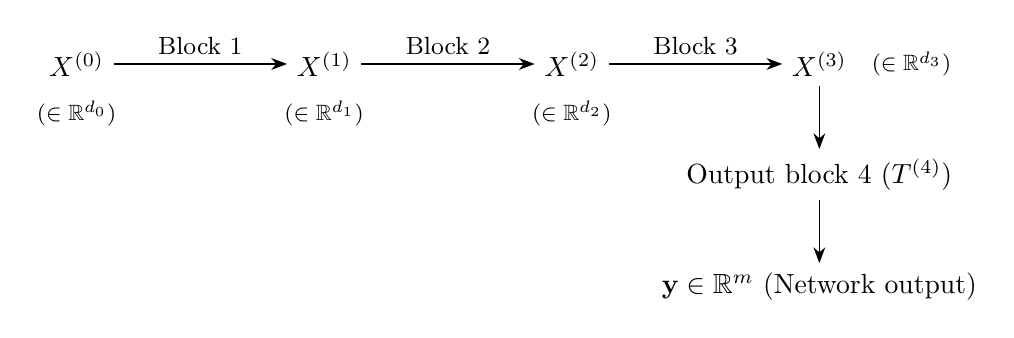
\begin{tikzpicture}[
    node distance=0.8cm and 2.2cm, % Vertical and horizontal node distances
    block/.style={font=\small}, % Style for block labels
    dim/.style={font=\footnotesize} % Style for dimension labels
  ]
    % Define nodes
    \node (X0)                                      {$X^{(0)}$};
    \node (L0) [below=0.07cm of X0, dim]             {$(\in \mathbb{R}^{d_0})$};
    \node (X1) [right=of X0]                        {$X^{(1)}$};
    \node (L1) [below=0.07cm of X1, dim]             {$(\in \mathbb{R}^{d_1})$};
    \node (X2) [right=of X1]                        {$X^{(2)}$};
    \node (L2) [below=0.07cm of X2, dim]             {$(\in \mathbb{R}^{d_2})$};
    \node (X3) [right=of X2]                        {$X^{(3)}$};
    \node (L3) [right=0.07cm of X3, dim]             {$(\in \mathbb{R}^{d_3})$};
    \node (OB) [below=of X3]                        {Output block 4 $(T^{(4)})$};
    \node (Y)  [below=of OB]                        {$\mathbf{y} \in \mathbb{R}^m$ (Network output)};

    % Draw arrows
    \draw[-{Stealth[length=2mm]}] (X0) -- node[above, block] {Block 1} (X1);
    \draw[-{Stealth[length=2mm]}] (X1) -- node[above, block] {Block 2} (X2);
    \draw[-{Stealth[length=2mm]}] (X2) -- node[above, block] {Block 3} (X3);
    \draw[-{Stealth[length=2mm]}] (X3) -- (OB); % Vertical arrow
    \draw[-{Stealth[length=2mm]}] (OB) -- (Y);  % Vertical arrow
\end{tikzpicture}
\end{center}
Here, $X^{(\ell)} = \mathbf{h}^{(\ell)}$ denotes the output vector of the $\ell$-th Sprecher block (we use both notations interchangeably for clarity in different contexts). Each block $T^{(\ell)}$ internally uses its own pair of shared splines $(\phi^{(\ell)}, \Phi^{(\ell)})$, mixing weights $\lambda^{(\ell)}$, and shift $\eta^{(\ell)}$. The final output block $T^{(4)}$ maps the representation $X^{(3)}$ to the final $m$-dimensional output $\mathbf{y}$ without subsequent summation.

\subsection{Illustrative expansions (scalar output)}
To further clarify the compositional structure for the scalar output case ($m=1$), we write out the full expansions for networks with $L=1, 2, 3$ hidden layers.

\subsubsection{Single hidden layer ($L=1$)}\label{sec:single_layer}
For a network with architecture $d_{\mathrm{in}}\to[d_1]\to1$ (i.e., $d_0=d_{\mathrm{in}}$), the network computes:
$$f(\mathbf{x}) = \sum_{q=0}^{d_1-1} \mathbf{h}^{(1)}_q = \sum_{q=0}^{d_1-1} \Phi^{(1)}\Biggl(\sum_{i=1}^{d_0} \lambda^{(1)}_{i}\,\phi^{(1)}\Bigl(x_i+\eta^{(1)}\,q\Bigr)+q\Biggr).$$
This precisely reproduces Sprecher's 1965 construction if we choose $d_1=2d_0+1$ and identify $\phi^{(1)}=\phi$, $\Phi^{(1)}=\Phi$, and $\lambda^{(1)}_{i} = \lambda_i$.

\subsubsection{Two hidden layers ($L=2$)}
Let the architecture be $d_0\to[d_1, d_2]\to1$. The intermediate output $\mathbf{h}^{(1)} \in \mathbb{R}^{d_1}$ is computed as:
$$\mathbf{h}^{(1)}_r=\Phi^{(1)}\Bigl(\sum_{i=1}^{d_0}\lambda^{(1)}_{i}\,\phi^{(1)}\Bigl(x_i+\eta^{(1)}\,r\Bigr)+r\Bigr),\quad r=0,\dots,d_1-1.$$
The second block computes $\mathbf{h}^{(2)} \in \mathbb{R}^{d_2}$ using $\mathbf{h}^{(1)}$ as input:
$$\mathbf{h}^{(2)}_q=\Phi^{(2)}\Bigl(\sum_{r=0}^{d_1-1}\lambda^{(2)}_{r}\,\phi^{(2)}\Bigl(\mathbf{h}^{(1)}_r+\eta^{(2)}\,q\Bigr)+q\Bigr),\quad q=0,\dots,d_2-1.$$
The final network output is the sum over the components of $\mathbf{h}^{(2)}$: $f(\mathbf{x})=\sum_{q=0}^{d_2-1}\mathbf{h}^{(2)}_q$. Substituting $\mathbf{h}^{(1)}$, the fully expanded form is:
\begin{equation}\label{eq:two-layer-restored}
f(\mathbf{x})=\sum_{q=0}^{d_2-1}\Phi^{(2)}\Biggl(\sum_{r=0}^{d_1-1}\lambda^{(2)}_{r}\,\phi^{(2)}\Biggl(\Phi^{(1)}\Biggl(\sum_{i=1}^{d_0}\lambda^{(1)}_{i}\,\phi^{(1)}\Bigl(x_i+\eta^{(1)}\,r\Bigr)+r\Biggr)+\eta^{(2)}\,q\Biggr)+q\Biggr).
\end{equation}

\subsubsection{Three hidden layers ($L=3$)}
Let the architecture be $d_0\to [d_1, d_2, d_3]\to1$. The recursive definition involves:
$$\begin{aligned}
\mathbf{h}^{(1)}_r &= \Phi^{(1)}\Bigl(\sum_{i=1}^{d_0}\lambda^{(1)}_{i}\,\phi^{(1)}\Bigl(x_i+\eta^{(1)}\,r\Bigr)+r\Bigr),\quad r=0,\dots,d_1-1,\\[1mm]
\mathbf{h}^{(2)}_s &= \Phi^{(2)}\Bigl(\sum_{r=0}^{d_1-1}\lambda^{(2)}_{r}\,\phi^{(2)}\Bigl(\mathbf{h}^{(1)}_r+\eta^{(2)}\,s\Bigr)+s\Bigr),\quad s=0,\dots,d_2-1,\\[1mm]
\mathbf{h}^{(3)}_q &= \Phi^{(3)}\Bigl(\sum_{s=0}^{d_2-1}\lambda^{(3)}_{s}\,\phi^{(3)}\Bigl(\mathbf{h}^{(2)}_s+\eta^{(3)}\,q\Bigr)+q\Bigr),\quad q=0,\dots,d_3-1.
\end{aligned}$$
The network output is $f(\mathbf{x})=\sum_{q=0}^{d_3-1}\mathbf{h}^{(3)}_q$. The equivalent nested formulation is:
\begin{multline}\label{eq:three-layer-restored}
f(\mathbf{x})=\sum_{q=0}^{d_3-1}\Phi^{(3)}\Biggl(\sum_{s=0}^{d_2-1}\lambda^{(3)}_{s}\,\phi^{(3)}\Biggl(\Phi^{(2)}\Biggl(\sum_{r=0}^{d_1-1}\lambda^{(2)}_{r}\,\phi^{(2)}\Biggl(\Phi^{(1)}\Biggl(\sum_{i=1}^{d_0}\lambda^{(1)}_{i}\,\phi^{(1)}\Bigl(x_i+\eta^{(1)}\,r\Bigr)+r\Biggr)\\
+\eta^{(2)}\,s\Biggr)+s\Biggr)+\eta^{(3)}\,q\Biggr)+q\Biggr).
\end{multline}

\begin{remark}
These expansions highlight the compositional nature where the output of one Sprecher block, which is a vector of transformed values, serves as the input to the next. Each transformation layer involves its own pair of shared splines and learnable parameters.
\end{remark}

\begin{remark}[Necessity of internal shifts]\label{rem:shiftneeded}
It is tempting to simplify the nested structures, for instance by removing the inner shift terms like $\eta^{(2)}q$ inside $\phi^{(2)}$ in \eqref{eq:two-layer-restored}, or $\eta^{(2)}s$ inside $\phi^{(2)}$ and $\eta^{(3)}q$ inside $\phi^{(3)}$ in \eqref{eq:three-layer-restored}. One might hypothesize that the outer splines $\Phi^{(\ell)}$ could absorb this shifting effect (yielding a single composite spline per Sprecher block). However, experiments (see Section \ref{sec:ablation_eta}) suggest that these internal shifts $\eta^{(\ell)}q$ (or $\eta^{(\ell)}s$) applied to the inputs of the $\phi^{(\ell)}$ splines are crucial for the effective functioning of deeper Sprecher Networks. Removing them significantly degrades performance. The precise theoretical reason for their necessity in the multi-layer case, beyond their presence in Sprecher's original single-layer formula, warrants further investigation.
\end{remark}

\subsection{Soft routing details}

The soft routing mechanism warrants detailed exposition as it represents a key innovation over fixed routing patterns. The temperature parameter $\tau$ plays a crucial role in the optimization dynamics:

\begin{itemize}
\item For low temperatures ($\tau \approx 1$), the routing weights are nearly uniform, allowing gradient flow through many paths but providing less structural bias.
\item For moderate temperatures ($\tau \approx 4$, our default), the routing maintains differentiability while creating preferences for specific connections.
\item For high temperatures ($\tau > 10$), the routing approaches discrete assignments, potentially leading to gradient vanishing on non-selected paths.
\end{itemize}

For the broadcasting case ($d_{\mathrm{in}} < d_{\mathrm{out}}$), each soft index $s_j$ for $j = 0, \ldots, d_{\mathrm{out}}-1$ indicates which input should primarily feed into output $j$:
$$R_{ij} = \frac{\exp(-\tau \cdot (s_j \cdot (d_{\mathrm{in}}-1) - i)^2)}{\sum_{k=0}^{d_{\mathrm{in}}-1} \exp(-\tau \cdot (s_j \cdot (d_{\mathrm{in}}-1) - k)^2)}$$

\begin{remark}[Regularization of soft indices]
To prevent soft indices from deviating too far from their initialization, an optional L2 regularization term can be added:
$$\mathcal{L}_{\text{reg}} = \lambda_{\text{reg}} \sum_{\ell} \left\|\mathbf{s}^{(\ell)} - \mathbf{s}^{(\ell)}_{\text{init}}\right\|_2^2$$
where $\mathbf{s}^{(\ell)}_{\text{init}}$ are the uniformly spaced initial values. This encourages the network to maintain reasonably distributed connections while allowing task-specific adaptations.
\end{remark}

\section{Comparison with related architectures}
To position Sprecher Networks accurately, we compare their core architectural features with Multi-Layer Perceptrons (MLPs), networks with learnable node activations (LANs/Adaptive-MLPs), and Kolmogorov-Arnold Networks (KANs).

\begin{table}[ht]
\centering
\caption{Architectural comparison of neural network families.}
\label{tab:arch_comparison}
\small % Use smaller font size if needed
\begin{tabular}{@{}lllll@{}}
\toprule
Feature                   & MLP                 & LAN / Adaptive-MLP & KAN                   & Sprecher Network (SN) \\ \midrule
\textbf{Learnable}        & Linear Weights      & Linear Weights     & Edge Splines          & Block Splines ($\phi, \Phi$) \\
\textbf{Components}       & (on edges)          & + Node Activations &                       & + Mixing Weights ($\lambda$) \\
                          &                     &                    &                       & + Shift Parameter ($\eta$) \\
\textbf{Fixed components}   & Node Activations    & ---                & Node Summation        & Node Summation (implicit) \\
                          &                     &                    &                       & + Fixed Shifts ($+q$) \\
\textbf{Location of}      & Nodes               & Nodes              & Edges                 & Blocks \\
\textbf{Non-linearity}    & (Fixed)             & (Learnable)        & (Learnable)           & (Shared, Learnable) \\
\textbf{Node operation}     & Apply $\sigma(\cdot)$ & Apply $\sigma_{\text{learn}}(\cdot)$ & $\sum (\text{inputs})$ & Implicit in Block Formula \\
\textbf{Parameter sharing}  & None (typically)    & Activations? (Maybe) & None (typically)      & Splines ($\phi, \Phi$) per block \\
\textbf{Residual design}    & Matrix projection   & Matrix projection  & None (typically)      & Soft routing \\
                          & $O(N^2)$ per skip   & $O(N^2)$ per skip  &                       & $O(N)$ per skip \\
\textbf{Theoretical basis}  & UAT                 & UAT                & KAT (inspired)        & KAS (Sprecher, direct) \\
\textbf{Param scaling}    & $O(L N^2)$          & $O(L N^2 + L N G)$ & $O(L N^2 G)$          & $O(L N + L G)$ \\
                          &                     & (Approx.)          &                       & (Approx.) \\
\bottomrule
\end{tabular}
\vspace{2mm}
\parbox{\textwidth}{\footnotesize \textit{Notes:} $L$=depth, $N$=average width, $G$=spline grid size/complexity. UAT=Universal Approx. Theorem, KAT=Kolmogorov-Arnold Theorem, KAS=Kolmogorov-Arnold-Sprecher. LAN details often follow KAN Appendix B \cite{liu2024kan}. All architectures may optionally include normalization layers; SNs apply normalization to entire block outputs rather than individual activations. For soft routing residuals, each connection contributes at most $2\max(d_{\mathrm{in}}, d_{\mathrm{out}})$ parameters (soft indices plus optional pooling weights), maintaining the linear scaling.
\textit{The parameter scaling notation uses $N$ to denote a typical or average layer width for simplicity, following \cite{liu2024kan}. For architectures with varying widths $d_\ell$, the $LN^2$ terms should be understood as $\sum_{\ell} d_{\ell-1}d_{\ell}$ (MLP, LAN), the $LN^2G$ term for KAN as $(\sum_{\ell} d_{\ell-1}d_{\ell})G$, and the $LN$ term for SN as $\sum_{\ell} d_{\ell-1}$ (since SN uses weight vectors, not matrices), where the sum is over the relevant blocks/layers, for precise counts.}}
\end{table}

Table \ref{tab:arch_comparison} summarizes the key distinctions between these architectures. MLPs learn edge weights with fixed node activations, LANs add learnable node activations to this structure, KANs move learnability entirely to edge splines while eliminating linear weights, and SNs concentrate learnability in shared block-level splines, block-level shifts, and mixing weights. The critical difference for SNs is their use of weight vectors rather than matrices, which fundamentally reduces the dependence on width from quadratic to linear. This architectural choice can be understood through an analogy with convolutional neural networks: just as CNNs achieve parameter efficiency and improved generalization by sharing weights across spatial locations, SNs share weights across output dimensions within each block. In CNNs, spatial shifts provide the necessary diversity despite weight sharing; in SNs, the shifts $\eta q$ and the additive term $+q$ play this diversifying role. This perspective reframes our architectural constraint not as a limitation, but as a principled form of weight sharing motivated by Sprecher's theorem, suggesting that SNs might be viewed as a ``convolutional'' approach to function approximation networks. While this weight sharing is theoretically justified for single-layer networks, its effectiveness in deep compositions remains an empirical finding that warrants further theoretical investigation. This combination of choices leads to SNs' distinctive parameter scaling of $O(L N + L G)$ compared to KANs' $O(L N^2 G)$.\footnote{The $O(LN)$ term includes contributions from mixing weights ($\lambda$), normalization parameters when used, and soft routing residual connections. Each residual connection contributes at most $2\max(d_{\mathrm{in}}, d_{\mathrm{out}})$ parameters (soft indices plus pooling weights), maintaining the linear scaling in width.}

{\color{red}Here, we provide a precise comparison between LANs and SNs. While the following proposition shows that SNs can be expressed as special cases of LANs with specific structural constraints, it is important to note that Sprecher's construction guarantees that this constrained form retains full expressivity in the single-layer case. This suggests that the extreme parameter sharing and structural constraints in SNs may serve as a beneficial inductive bias rather than a limitation.}

{\color{red}\begin{definition}
A LAN is an MLP with learnable activation. More precisely, the model is defined as: 
$$
f(\mathbf{x}) = A^{(L)} \circ \sigma^{(L-1)} \circ A^{(L-1)} \circ \sigma^{(L-2)} \circ \cdots \circ \sigma^{(1)} \circ A^{(1)} (\mathbf{x}),
$$
where $A^{(k)} \colon \mathbb{R}^{d_{k-1}} \rightarrow \mathbb{R}^{d_k}$ is an affine map, and $\sigma^{(k)} \colon \mathbb{R} \rightarrow \mathbb{R}  $ is the activation function (applied coordinate-wise). In an MLP, the trainable parameters are the weights $W^{(k)}$ and biases $b^{(k)}$ of $A^{(k)}(\mathbf{x}) = W^{(k)}\mathbf{x} + b^{(k)}$ for $k = 1, \ldots, L$. In a LAN, $\sigma$ contains additional trainable parameters, e.g., the coefficients of a spline.
\end{definition}}

{\color{red}\begin{remark}[Note on weight structure]
The following proposition uses matrix weights $\lambda_{i,q}^{(\ell)}$ to establish the connection between SNs and LANs. However, the architecture we propose and analyze throughout this paper uses vector weights $\lambda_i^{(\ell)}$ (following Sprecher's original formulation), where the same weights are shared across all output dimensions. This vector version represents an even more constrained special case of the LAN formulation shown below. The practical SN architecture with vector weights would require the weight matrices in the proposition to have repeated rows, i.e., $\lambda_{i,q}^{(\ell)} = \lambda_i^{(\ell)}$ for all $q$. This constraint is fundamental to maintaining the "true Sprecher" structure and achieving the characteristic $O(LN)$ parameter scaling.
\end{remark}}

{\color{red}\begin{prop} \label{prop:SNareLAN}
    An SN with matrix weights (cf. \eqref{eq:defsn}) is a LAN, where: 
    \begin{itemize}
        \item in odd layers $k = 2\ell - 1$, the weight matrix $W^{(k)} \in \mathbb{R}^{d_\ell d_{\ell-1} \times d_{\ell-1}}$ is fixed to  $[I | \cdots | I]^\top$, where $I$ is the $d_{\ell-1} \times d_{\ell-1}$ identity matrix, the bias vector has only one learnable parameter $\eta^{(\ell)}$ and is structured as $b^{(k)} = \eta^{(\ell)}(0,\ldots,0, 1, \ldots, 1, \ldots, d_{\ell}-1, \ldots, d_{\ell}-1)^\top \in \mathbb{R}^{d_\ell d_{\ell-1}}$, and the activation is $\sigma^{(k)} = \phi^{(\ell)}$, 
        \item in even layers $k = 2\ell $, the learnable weight matrix $W^{(k)} \in \mathbb{R}^{d_\ell \times d_\ell d_{\ell-1}}$ is structured as
        \begin{align*}
            \begin{bmatrix}
                \lambda_{1,0}^{(\ell)} & \cdots & \lambda_{d_{\ell-1},0}^{(\ell)} & 0 &&& \cdots &&&0 \\
               0  &\cdots & 0 & \lambda_{1,1}^{(\ell)} & \cdots & \lambda_{d_{\ell-1},1}^{(\ell)} & 0 && \cdots & 0 \\
               &&&&&& \ddots \\
               0 &&&\cdots &&&0&\lambda_{1,d_\ell-1}^{(\ell)} & \cdots & \lambda_{d_{\ell-1},d_\ell-1}^{(\ell)}
            \end{bmatrix},
        \end{align*} 
        the bias is fixed to $b^{(k)} = (0,\ldots, d_\ell-1)^\top \in \mathbb{R}^{d_\ell}$, and the activation is $\sigma^{(k)} = \Phi^{(\ell)}$. 
    \end{itemize}
\end{prop}
\begin{proof}
    Follows immediately by inspecting \eqref{eq:SN}.
\end{proof}
\begin{remark}[Understanding the LAN representation]
The representation of SNs as LANs in Proposition~\ref{prop:SNareLAN} uses an expanded 
intermediate state space. Each Sprecher block is decomposed into two LAN layers:
\begin{itemize}
\item The first layer expands the input $\mathbf{h}^{(\ell-1)} \in \mathbb{R}^{d_{\ell-1}}$ 
to $\mathbb{R}^{d_\ell d_{\ell-1}}$ by creating $d_\ell$ shifted copies, where the 
$(q \cdot d_{\ell-1} + i)$-th component contains $\phi^{(\ell)}(h^{(\ell-1)}_i + \eta^{(\ell)} q)$.
\item The second layer applies the mixing weights $\lambda^{(\ell)}_{i,q}$ to select and sum 
the appropriate components for each output $q$, adds the shift $q$, and applies $\Phi^{(\ell)}$.
\end{itemize}
This construction shows that while SNs can be expressed within the LAN framework, they 
represent a highly structured special case with specific weight patterns and an expanded 
intermediate dimension of $O(d_{\ell-1} d_\ell)$ between each pair of SN layers.
\end{remark}
While this proposition shows that SNs are special cases of LANs with specific structural constraints, Sprecher's construction guarantees that this constrained form retains full expressivity. In Sprecher's original construction, $\eta$ can be chosen as a universal constant rather than a learnable parameter. This, combined with Proposition \ref{prop:SNareLAN}, implies that LANs do not lose expressivity when constraining biases to specific structured forms.}
%    \item open problem: theoretical comparison of the models, e.g., dimension of their neuromanifolds? (hard in general, but possible in concrete example)
\textcolor{red}{\begin{figure}[h!]
    \centering  
\begin{tikzcd}[ampersand replacement=\&]
    \& \textnormal{LAN} \\
    \textnormal{MLP} \&\& \textnormal{SN}
    \arrow[hook, from=2-1, to=1-2]
    \arrow[hook', from=2-3, to=1-2]
\end{tikzcd}
    \caption{\textcolor{red}{Diagram illustrating the dependencies between the models, in terms of learnable parameters. MLPs are LANs with fixed activation function, while SNs are LANs with a particular parameter structure (Proposition \ref{prop:SNareLAN}).}}
    \label{fig:enter-label}
\end{figure}}

\textcolor{red}{\begin{remark}[Domain considerations]
The above proposition assumes that the spline functions $\phi^{(\ell)}$ can handle inputs outside their original domain $[0,1]$, which may arise due to the shifts $\eta^{(\ell)}q$. While Sprecher's theoretical construction extends $\phi$ appropriately, practical implementations typically compute exact theoretical bounds for all spline domains based on the network structure, ensuring that all evaluations fall within the spline's operating range through dynamic domain updates.
\end{remark}}

\section{Parameter counting and efficiency as a trade-off}
A key consequence of adhering to the vector-based weighting scheme inspired by Sprecher's formula is a dramatic reduction in parameters compared to standard architectures. This represents a strong architectural constraint that may serve as either a beneficial inductive bias or a limitation, depending on the target function class. The specific design of SNs, particularly the sharing of splines and use of weight vectors rather than matrices, leads to a distinctive parameter scaling that warrants careful analysis.

Let's assume a network of depth $L$ (meaning $L$ hidden layers, thus $L$ blocks for scalar output or $L+1$ for vector output), with an average layer width $N$. We denote the input dimension as $N_{in}$ when it differs significantly from the hidden layer widths. Let $G$ be the number of intervals used for the piecewise-linear splines (implying $G+1$ knots). For simplicity, we approximate the number of parameters per spline as $O(G)$.

The parameter counts for different architectures scale as follows. MLPs primarily consist of linear weight matrices, leading to a total parameter count dominated by these weights, scaling as $O(L N^2)$. LANs (Adaptive-MLPs) have both linear weights ($O(L N^2)$) and learnable activations; if each of the $N$ nodes per layer has a learnable spline, this adds $O(L N G)$ parameters, for a total of $O(L N^2 + L N G)$. KANs replace linear weights with learnable edge splines, with $O(N^2)$ edges between layers. If each edge has a spline with $O(G)$ parameters, the total count per layer is $O(N^2 G)$, leading to an overall scaling of $O(L N^2 G)$.

Sprecher Networks have a fundamentally different structure. Each block $\ell$ contains mixing weights $\lambda^{(\ell)}$ with $O(d_{\ell-1})$ parameters, where $d_{\ell-1}$ is the input dimension to that block (crucially, these are vectors, not matrices), shared splines $\phi^{(\ell)}, \Phi^{(\ell)}$ with $2 \times O(G) = O(G)$ parameters per block independent of $N$, and a shift parameter $\eta^{(\ell)}$ with $O(1)$ parameter per block. When normalization is used, each block may have an associated normalization layer adding $O(N)$ parameters (specifically $2N$ for the affine transformation). When residual connections are used with soft routing, they add at most $O(\max(d_{\ell-1}, d_\ell))$ parameters per block: soft indices plus any dimension-specific weights for the pooling case. Summing over $L$ (or $L+1$) blocks, the total parameter count scales approximately as $O(LN + LG + L)$, where the linear dependence on $N$ now includes mixing weights, optional normalization parameters, and soft routing parameters.

This scaling reveals the crucial trade-off: SNs achieve a reduction from $O(LN^2)$ to $O(LN)$ in the width-dependent term by using weight vectors rather than matrices. Additionally, in KANs, the spline complexity $G$ multiplies the $N^2$ term ($O(L N^2 G)$), while in SNs, due to spline sharing within blocks, it appears as an additive term ($O(L G)$). This suggests potential for significant parameter savings, particularly when high spline resolution ($G$) is required for accuracy or when the layer width ($N$) is moderate to large.

This extreme parameter sharing represents a fundamental architectural bet: that the structure imposed by Sprecher's theorem, using only weight vectors with output diversity through shifts, provides a beneficial inductive bias that outweighs the reduction in parameter flexibility. The empirical observation that training remains feasible (albeit slower) with vector weights suggests this bet may be justified for certain function classes. Moreover, viewing this constraint through the lens of weight sharing in CNNs provides a new perspective: both architectures sacrifice parameter flexibility for a structured representation that has proven effective in practice, though for SNs the theoretical justification comes from Sprecher's theorem rather than domain-specific intuitions about spatial invariance. Whether this constraint serves as beneficial regularization or harmful limitation likely depends on the specific problem domain and the alignment between the target function's structure and the inductive bias imposed by the SN architecture.

{\color{red}\subsection{Illustrative parameter comparisons (hypothetical examples)}}
\textcolor{red}{We present parameter count comparisons based on architectures reported in \cite{liu2024kan} to illustrate the potential parameter efficiency of SNs. Note that these examples are hypothetical – while the KAN architectures are from their paper, the SN results are theoretical projections that require empirical validation. Optimal architectures for SNs may differ from those of KANs due to the shared spline structure.}

{\color{red}\paragraph{PDE solving example (KAN Ref \S 3.4):}}
\textcolor{red}{KAN architecture $[2, 10, 1]$, reported effective. $N_{in}=2, N_{hid}=10, N_{out}=1$.}
\begin{itemize}
    \item \textcolor{red}{\textbf{KAN (est.):} $(2\times10 + 10\times1) = 30$ edges/splines. KANs use B-splines with $G=20$ intervals, $k=3$ ($G+k \approx 23$ params/spline). Total KAN params $\approx 30 \times 23 = 690$.}
    \item \textcolor{red}{\textbf{SN (hypothetical):} Architecture $2 \to [10] \to 1$. $L=1$ hidden layer, scalar output means $L=1$ block total. SNs use piecewise linear splines with $G=20$ intervals ($G+1 = 21$ params/spline). Shared splines: $2 \times 21 = 42$. Mixing weights: $d_0 = 2$ (vector weights). Shift $\eta^{(1)}$: $1$. Total SN params $\approx 42 + 2 + 1 = 45$.}
    \item \textcolor{red}{\textbf{Potential advantage:} For equivalent structure, theoretical reduction factor $\approx 15$x (45 vs 690). Actual performance requires empirical validation.}
\end{itemize}

{\color{red}\paragraph{Knot theory example (KAN Ref \S 4.3):}}
\textcolor{red}{Pruned KAN $[17, 1, 14]$, with B-splines using $G=3$ intervals, $k=3$ ($G+k \approx 6$ params/spline).}
\begin{itemize}
    \item \textcolor{red}{\textbf{KAN (est.):} $(17\times1 + 1\times14) = 31$ edges/splines. Total KAN params $\approx 31 \times 6 = 186$.}
    \item \textcolor{red}{\textbf{SN (hypothetical):} Architecture $17 \to [1] \to 14$. $L=1$ hidden layer, vector output means $L+1=2$ blocks total. Using piecewise linear splines with $G=3$ intervals: $2(L+1) \times (G+1) = 4 \times 4 = 16$. Mixing weights: $d_0 + d_1 = 17 + 1 = 18$ (vector weights). Shifts $\eta^{(1)}, \eta^{(2)}$: $2$. Total SN params $\approx 16 + 18 + 2 = 36$.}
    \item \textcolor{red}{\textbf{Potential advantage:} Theoretical reduction factor $\approx 5.2$x (36 vs 186). The narrow intermediate dimension $d_1=1$ might pose challenges for SN training.}
\end{itemize}

\textcolor{red}{These calculations illustrate the dramatic parameter reduction possible with SNs, but they also highlight a crucial practical consideration: the optimal architecture for SNs likely differs substantially from that of MLPs or KANs. With vector weights providing only linear scaling in width, SNs may require wider or deeper architectures to achieve comparable expressivity. The art of architecture selection for SNs involves balancing the parameter efficiency against the need for sufficient expressivity: a trade-off that remains poorly understood and likely depends strongly on the problem domain. Early empirical evidence suggests that SNs excel when the target function aligns well with their compositional, shift-based structure, but struggle when forced to approximate functions that require truly independent processing of different output dimensions.}

\section{Theoretical aspects and open questions}\label{sec:universality}

\subsection{Relation to Sprecher (1965) and universality}
As shown in Section \ref{sec:single_layer}, a single-layer ($L=1$) Sprecher Network with input dimension $d_0=n$ and output dimension $d_1 = 2n+1$, when configured with appropriate (potentially fixed) weights $\lambda^{(1)}_{i} = \lambda_i$ and shift $\eta^{(1)} = \eta$, directly reproduces Sprecher's 1965 formula \eqref{eq:sprecher_original}.
Sprecher proved that for any continuous function $f:[0,1]^n \to \mathbb{R}$, there exist a suitable monotonic $\phi$, a continuous $\Phi$, and constants $\lambda_p, \eta$ such that this representation holds \cite{sprecher1965}. This immediately implies:

\begin{theorem}[Universality of single-layer SNs]
For any dimension $n \ge 1$ and any continuous function $f: [0,1]^n \to \mathbb{R}$, and any $\epsilon > 0$, there exists a single-layer Sprecher Network with architecture $n \to [2n+1] \to 1$, using sufficiently flexible (e.g., high knot count) continuous splines $\phi^{(1)}$ (monotonic) and $\Phi^{(1)}$, and appropriate parameters $\lambda^{(1)}, \eta^{(1)}$, such that the network output $\hat{f}(\mathbf{x})$ satisfies $\sup_{\mathbf{x} \in [0,1]^n} |f(\mathbf{x}) - \hat{f}(\mathbf{x})| < \epsilon$.
\end{theorem}
Thus, single-layer SNs inherit the universal approximation property directly from Sprecher's constructive proof for functions defined on the unit hypercube. Notably, our use of weight vectors $\lambda_i$ rather than matrices $\lambda_{i,q}$ maintains complete fidelity to Sprecher's original formulation, which used constants $\lambda_p$ depending only on the input index. This is more than a historical curiosity: Sprecher's proof demonstrates that this constrained form is sufficient for universal approximation, suggesting that the additional parameters in a full matrix formulation may be redundant. The vector formulation enforces a specific structure where all output dimensions share the same linear combination of transformed inputs, with diversity arising solely from the shifts, a constraint that Sprecher showed does not limit expressivity in the single-layer case.

While universality guarantees that an approximation exists, it doesn't quantify how the error behaves as the approximating functions (splines) become more refined. The following lemmas and theorem address the approximation rate achievable by replacing the ideal continuous functions in the Sprecher structure with finite-resolution splines, assuming such an ideal network exists for the target function $f$.

\begin{remark}[Piecewise linear splines in practice]
While the following theoretical analysis considers general degree-$k$ splines for completeness, the Sprecher Network architecture as implemented specifically requires piecewise linear splines ($k=1$). This constraint is not merely an implementation choice but a fundamental requirement for the efficient domain computation algorithm described in Section~\ref{sec:theoretical_domains}. 

For piecewise linear splines, the extrema occur only at knot points, enabling exact output range computation in $O(G)$ time by simply evaluating the spline at its knots. Higher-degree splines would require finding critical points through differentiation and root-finding in each interval, making the domain propagation algorithm computationally prohibitive and potentially numerically unstable.

The following analysis with general $k$ is provided to illustrate how approximation rates would scale with spline degree in principle, but readers should understand that $k=1$ is architecturally required for the domain management system that is central to SNs' practical implementation.
\end{remark}

\begin{lemma}[Single block approximation]\label{lem:single_block}
Consider a single Sprecher block $T: \mathbb{R}^{d_{in}} \to \mathbb{R}^{d_{out}}$ defined by
$$T(\mathbf{z})_q = \Phi\left(\sum_{i=1}^{d_{in}} \lambda_{i} \phi(z_i + \eta q) + q\right), \quad q = 0, \ldots, d_{out}-1$$
where $\phi \in C^{k+1}(\mathbb{R})$ is monotonic, $\Phi \in C^{k+1}(\mathbb{R})$, $|\lambda_{i}| \leq \Lambda$, and $\eta > 0$.

Suppose the input satisfies $\mathbf{z} \in \mathcal{B}_{in} := [-B_{in}, B_{in}]^{d_{in}}$. Define:
\begin{itemize}
\item $I_\phi := [-B_{in} - \eta(d_{out}-1), B_{in} + \eta(d_{out}-1)]$ (domain containing all possible arguments to $\phi$)
\item $I_\Phi := [-R_{out}, R_{out}]$ where $R_{out} := \Lambda d_{in} \|\phi\|_{L^\infty(I_\phi)} + d_{out}$ (domain containing all possible arguments to $\Phi$)
\end{itemize}

Let $\hat{\phi}$ be a monotonic spline of degree $k$ with $G_\phi$ uniformly spaced knots on $I_\phi$, and $\hat{\Phi}$ be a spline of degree $k$ with $G_\Phi$ uniformly spaced knots on $I_\Phi$. Note that while this theorem assumes degree-$k$ splines for generality, practical implementations often use piecewise linear splines ($k=1$) for computational efficiency. If
$$\|\phi - \hat{\phi}\|_{L^\infty(I_\phi)} \leq \frac{\|\phi^{(k+1)}\|_{L^\infty(I_\phi)}}{(k+1)!} \left(\frac{|I_\phi|}{G_\phi}\right)^{k+1}$$
$$\|\Phi - \hat{\Phi}\|_{L^\infty(I_\Phi)} \leq \frac{\|\Phi^{(k+1)}\|_{L^\infty(I_\Phi)}}{(k+1)!} \left(\frac{|I_\Phi|}{G_\Phi}\right)^{k+1}$$
then the approximate block $\hat{T}$ using $\hat{\phi}, \hat{\Phi}$ satisfies
$$\sup_{\mathbf{z} \in \mathcal{B}_{in}} \|T(\mathbf{z}) - \hat{T}(\mathbf{z})\|_\infty \leq K_T \max\left\{\left(\frac{|I_\phi|}{G_\phi}\right)^{k+1}, \left(\frac{|I_\Phi|}{G_\Phi}\right)^{k+1}\right\}$$
where 
$$K_T := \frac{L_\Phi \Lambda d_{in} \|\phi^{(k+1)}\|_{L^\infty(I_\phi)} + \|\Phi^{(k+1)}\|_{L^\infty(I_\Phi)}}{(k+1)!}$$
and $L_\Phi$ is the Lipschitz constant of $\Phi$ on $I_\Phi$.
\end{lemma}

\begin{proof}
Fix $\mathbf{z} \in \mathcal{B}_{in}$ and $q \in \{0, \ldots, d_{out}-1\}$. Define:
$$s_q := \sum_{i=1}^{d_{in}} \lambda_{i} \phi(z_i + \eta q) + q, \quad \hat{s}_q := \sum_{i=1}^{d_{in}} \lambda_{i} \hat{\phi}(z_i + \eta q) + q$$

Since $z_i \in [-B_{in}, B_{in}]$ and $0 \leq \eta q \leq \eta (d_{out}-1)$, we have $z_i + \eta q \in I_\phi$. Thus:
\begin{align*}
|s_q - \hat{s}_q| &= \left|\sum_{i=1}^{d_{in}} \lambda_{i} [\phi(z_i + \eta q) - \hat{\phi}(z_i + \eta q)]\right|\\
&\leq \sum_{i=1}^{d_{in}} |\lambda_{i}| \cdot \|\phi - \hat{\phi}\|_{L^\infty(I_\phi)}\\
&\leq \Lambda d_{in} \cdot \frac{\|\phi^{(k+1)}\|_{L^\infty(I_\phi)}}{(k+1)!} \left(\frac{|I_\phi|}{G_\phi}\right)^{k+1}
\end{align*}

Moreover, $|s_q| \leq \Lambda d_{in} \|\phi\|_{L^\infty(I_\phi)} + |q| \leq \Lambda d_{in} \|\phi\|_{L^\infty(I_\phi)} + d_{out} = R_{out}$, so $s_q \in I_\Phi$. Similarly, since $\hat{\phi}$ is bounded on $I_\phi$ (as a continuous function on a compact set), $\hat{s}_q \in I_\Phi$ for sufficiently large $G_\phi$.

Now:
\begin{align*}
|T(\mathbf{z})_q - \hat{T}(\mathbf{z})_q| &= |\Phi(s_q) - \hat{\Phi}(\hat{s}_q)|\\
&\leq |\Phi(s_q) - \Phi(\hat{s}_q)| + |\Phi(\hat{s}_q) - \hat{\Phi}(\hat{s}_q)|\\
&\leq L_\Phi |s_q - \hat{s}_q| + \|\Phi - \hat{\Phi}\|_{L^\infty(I_\Phi)}\\
&\leq L_\Phi \Lambda d_{in} \frac{\|\phi^{(k+1)}\|_{L^\infty(I_\phi)}}{(k+1)!} \left(\frac{|I_\phi|}{G_\phi}\right)^{k+1} + \frac{\|\Phi^{(k+1)}\|_{L^\infty(I_\Phi)}}{(k+1)!} \left(\frac{|I_\Phi|}{G_\Phi}\right)^{k+1}
\end{align*}

Taking the maximum over $q$ and $\mathbf{z}$ gives the result.
\end{proof}

\begin{lemma}[Error composition]\label{lem:error_composition}
Consider an $L$-block Sprecher network where block $\ell$ has approximation constant $K_{T^{(\ell)}}$ and Lipschitz constant $L_{T^{(\ell)}}$ (viewing the block as a function $T^{(\ell)}: \mathbb{R}^{d_{\ell-1}} \to \mathbb{R}^{d_\ell}$). Let $E_\ell$ denote the worst-case error after block $\ell$:
$$E_\ell := \sup_{\mathbf{x} \in [0,1]^n} \|\mathbf{h}^{(\ell)}(\mathbf{x}) - \hat{\mathbf{h}}^{(\ell)}(\mathbf{x})\|_\infty$$

Then:
\begin{equation}\label{eq:error_composition_result}
E_\ell \leq \sum_{j=1}^{\ell} \left(\prod_{m=j+1}^{\ell} L_{T^{(m)}}\right) K_{T^{(j)}} \varepsilon_j
\end{equation}
where $\varepsilon_j$ is the approximation error bound for block $j$ from Lemma \ref{lem:single_block}, and the empty product equals 1.
\end{lemma}

\begin{proof}
We proceed by induction. For $\ell = 1$, we have $E_1 \leq K_{T^{(1)}} \varepsilon_1$ directly from Lemma \ref{lem:single_block}.

Assume the result holds for $\ell-1$. For any $\mathbf{x} \in [0,1]^n$:
\begin{align*}
\|\mathbf{h}^{(\ell)}(\mathbf{x}) - \hat{\mathbf{h}}^{(\ell)}(\mathbf{x})\|_\infty &= \|T^{(\ell)}(\mathbf{h}^{(\ell-1)}(\mathbf{x})) - \hat{T}^{(\ell)}(\hat{\mathbf{h}}^{(\ell-1)}(\mathbf{x}))\|_\infty\\
&\leq \|T^{(\ell)}(\mathbf{h}^{(\ell-1)}(\mathbf{x})) - T^{(\ell)}(\hat{\mathbf{h}}^{(\ell-1)}(\mathbf{x}))\|_\infty \\
&\quad + \|T^{(\ell)}(\hat{\mathbf{h}}^{(\ell-1)}(\mathbf{x})) - \hat{T}^{(\ell)}(\hat{\mathbf{h}}^{(\ell-1)}(\mathbf{x}))\|_\infty\\
&\leq L_{T^{(\ell)}} \|\mathbf{h}^{(\ell-1)}(\mathbf{x}) - \hat{\mathbf{h}}^{(\ell-1)}(\mathbf{x})\|_\infty + K_{T^{(\ell)}} \varepsilon_\ell\\
&\leq L_{T^{(\ell)}} E_{\ell-1} + K_{T^{(\ell)}} \varepsilon_\ell
\end{align*}
Substituting the induction hypothesis completes the proof.
\end{proof}

\begin{theorem}[Spline approximation rate for Sprecher Networks]\label{thm:sprecher_rate}
Let $f:[0,1]^n \to \mathbb{R}$ be realized by an ideal $L$-block Sprecher network with scalar output. Assume:
\begin{enumerate}[label=\textup{(\roman*)}]
\item Each $\phi^{(\ell)}, \Phi^{(\ell)} \in C^{k+1}$ on their respective domains.
\item Each block satisfies $|\lambda_{i}^{(\ell)}| \leq \Lambda$ and has shift parameter $\eta^{(\ell)} > 0$.
\item The network propagates through bounded sets: $\mathbf{h}^{(\ell)}(\mathbf{x}) \in [-B_\ell, B_\ell]^{d_\ell}$ for all $\mathbf{x} \in [0,1]^n$.
\end{enumerate}

For each block $\ell$, approximate $\phi^{(\ell)}$ and $\Phi^{(\ell)}$ with degree-$k$ splines using $G_\phi^{(\ell)}$ and $G_\Phi^{(\ell)}$ knots respectively. Then:
$$\sup_{\mathbf{x} \in [0,1]^n} |f(\mathbf{x}) - \hat{f}(\mathbf{x})| \leq d_L \sum_{j=1}^{L} \left(\prod_{m=j+1}^{L} L_{T^{(m)}}\right) K_{T^{(j)}} \varepsilon_j$$
where:
\begin{itemize}
\item $\varepsilon_j = \max\left\{\left(\frac{2B_{j-1} + 2\eta^{(j)}(d_j-1)}{G_\phi^{(j)}}\right)^{k+1}, \left(\frac{2R_j}{G_\Phi^{(j)}}\right)^{k+1}\right\}$
\item $R_j = \Lambda d_{j-1} \|\phi^{(j)}\|_{L^\infty} + d_j$
\item $K_{T^{(j)}} = \frac{L_{\Phi^{(j)}} \Lambda d_{j-1} \|\phi^{(j)}{}^{(k+1)}\|_{L^\infty} + \|\Phi^{(j)}{}^{(k+1)}\|_{L^\infty}}{(k+1)!}$
\item $L_{T^{(m)}} = L_{\Phi^{(m)}} \Lambda d_{m-1} L_{\phi^{(m)}}$ (Lipschitz constant of block $m$)
\end{itemize}

If all blocks use the same number of knots $G$ (i.e., $G_\phi^{(\ell)}=G_\Phi^{(\ell)}=G$ for all $\ell$), the error scales as $O(G^{-(k+1)})$ with constants that may grow exponentially with depth $L$.
\end{theorem}

\begin{proof}
By Lemma \ref{lem:single_block}, each block $\ell$ can be approximated with error bounded by $K_{T^{(\ell)}} \varepsilon_\ell$. By Lemma \ref{lem:error_composition}, the error after $L$ blocks is bounded by the sum given in \eqref{eq:error_composition_result}.

For the scalar output case, we have:
\begin{align*}
|f(\mathbf{x}) - \hat{f}(\mathbf{x})| &= \left|\sum_{q=0}^{d_L-1} h_q^{(L)}(\mathbf{x}) - \sum_{q=0}^{d_L-1} \hat{h}_q^{(L)}(\mathbf{x})\right|\\
&\leq \sum_{q=0}^{d_L-1} |h_q^{(L)}(\mathbf{x}) - \hat{h}_q^{(L)}(\mathbf{x})|\\
&\leq d_L \|\mathbf{h}^{(L)}(\mathbf{x}) - \hat{\mathbf{h}}^{(L)}(\mathbf{x})\|_\infty\\
&\leq d_L E_L
\end{align*}
Substituting the bound for $E_L$ gives the result.
\end{proof}

\begin{remark}[Monotonic spline approximation]
The approximation rates in Lemma \ref{lem:single_block} assume we can achieve standard spline approximation rates while maintaining monotonicity for $\phi^{(\ell)}$. While the theoretical analysis considers general degree-$k$ splines, practical implementations typically use piecewise linear splines ($k=1$) with a log-space parameterization that maintains monotonicity by construction. For piecewise linear splines approximating smooth functions, the approximation rate becomes $O(G^{-2})$.
\end{remark}

\begin{remark}[Dependence on depth]
The constant in the error bound depends on the layer dimensions $d_\ell$ and the Lipschitz constants $L_\phi^{(\ell)}, L_\Phi^{(\ell)}$ through the factors $L_{T^{(m)}}$. If these factors are consistently greater than 1, the constant can grow exponentially with depth $L$. This highlights a potential challenge for approximation with very deep networks, similar to error bounds seen in other deep learning contexts.
\end{remark}

\subsection{Vector-valued functions and deeper extensions}
For vector-valued functions $f: [0,1]^n \to \mathbb{R}^m$ with $m>1$, our construction appends an $(L+1)$-th block without final summation. While intuitively extending the representation, the universality of this specific construction is not directly covered by Sprecher's original theorem. The composition of multiple Sprecher blocks to create deep networks represents a natural but theoretically uncharted extension of Sprecher's construction. While single-layer universality is guaranteed, the expressive power of deep SNs remains an open question with several competing hypotheses. Depth might provide benefits analogous to those in standard neural networks: enabling more efficient representation of compositional functions, creating a more favorable optimization landscape despite the constrained parameter space, or allowing the network to gradually transform inputs into representations that are progressively easier to process. Alternatively, the specific constraints of the SN architecture might interact with depth in unexpected ways, either amplifying the benefits of the structured representation or creating new challenges not present in single-layer networks.

\begin{conjecture}[Vector-valued Sprecher Representation]\label{conj:vector}
Let $n, m \in \mathbb{N}$ with $m > 1$, and let $f:[0,1]^n \to \mathbb{R}^m$ be any continuous function. Then for any $\epsilon > 0$, there exists a Sprecher Network with architecture $n \to [d_1] \to m$ (using $L=1$ hidden block of width $d_1 \ge 2n+1$ and one output block), with sufficiently flexible continuous splines $\phi^{(1)}, \Phi^{(1)}, \phi^{(2)}, \Phi^{(2)}$ ($\phi^{(1)}, \phi^{(2)}$ monotonic) and appropriate parameters $\lambda^{(1)}, \eta^{(1)}, \lambda^{(2)}, \eta^{(2)}$, such that the network output $\hat{f}(\mathbf{x})$ satisfies $\sup_{\mathbf{x} \in [0,1]^n} \|f(\mathbf{x}) - \hat{f}(\mathbf{x})\|_{\mathbb{R}^m} < \epsilon$.
\end{conjecture}

Furthermore, stacking multiple Sprecher blocks ($L > 1$) creates deeper networks. It is natural to hypothesize that these deeper networks also possess universal approximation capabilities, potentially offering advantages in efficiency or learning dynamics for certain function classes, similar to depth advantages observed in MLPs.

\begin{conjecture}[Deep universality]\label{conj:deep_universal}
For any input dimension $n \ge 1$, any number of hidden blocks $L \ge 1$, and any continuous function $f: [0,1]^n \to \mathbb{R}$ (or $f: [0,1]^n \to \mathbb{R}^m$), and any $\epsilon > 0$, there exists a Sprecher Network with architecture $n \to [d_1, \dots, d_L] \to 1$ (or $\to m$), provided the hidden widths $d_1, \dots, d_L$ are sufficiently large (e.g., perhaps $d_\ell \ge 2 d_{\ell-1} + 1$ is sufficient, although likely not necessary), with sufficiently flexible continuous splines $\phi^{(\ell)}, \Phi^{(\ell)}$ and appropriate parameters $\lambda^{(\ell)}, \eta^{(\ell)}$, such that the network output $\hat{f}(\mathbf{x})$ satisfies $\sup_{\mathbf{x} \in [0,1]^n} |f(\mathbf{x}) - \hat{f}(\mathbf{x})| < \epsilon$ (or the vector norm equivalent).
\end{conjecture}

Proving Conjectures \ref{conj:vector} and \ref{conj:deep_universal} rigorously would require analyzing the compositional properties and ensuring that the range of intermediate representations covers the domain needed by subsequent blocks, potentially involving careful control over the spline ranges and the effect of the shifts $\eta^{(\ell)}$.

\subsection{Theoretical properties of soft routing}
The soft routing mechanism introduces interesting theoretical questions about the expressivity of networks with learnable, continuous routing versus fixed patterns.

\begin{remark}[Soft routing as continuous relaxation]
The soft routing mechanism can be viewed as learning a continuous relaxation of permutation matrices. For the pooling case where $d_{\mathrm{in}} > d_{\mathrm{out}}$, the routing matrix $R$ satisfies:
\begin{itemize}
    \item Row-stochasticity: $\sum_{j=0}^{d_{\mathrm{out}}-1} R_{ij} = 1$ for all $i$
    \item Non-negativity: $R_{ij} \geq 0$ for all $i,j$
    \item Smoothness: $R_{ij}$ is differentiable with respect to the soft indices $s_i$
\end{itemize}

As the temperature $\tau \to \infty$, the soft assignments approach hard assignments, recovering a form similar to discrete routing but with learned positions. Conversely, as $\tau \to 0$, the assignments become uniform, equally distributing each input across all outputs.
\end{remark}

\begin{conjecture}[Expressivity of soft routing]
For any continuous residual function $r: \mathbb{R}^{d_{\mathrm{in}}} \to \mathbb{R}^{d_{\mathrm{out}}}$ and any $\epsilon > 0$, there exist soft routing parameters (indices $s$, temperature $\tau$, and weights $w$) such that the soft routing residual approximates $r$ within $\epsilon$ on any bounded domain.
\end{conjecture}

This conjecture suggests that soft routing does not limit the expressivity of residual connections despite using only $O(\max(d_{\mathrm{in}}, d_{\mathrm{out}}))$ parameters instead of $O(d_{\mathrm{in}} \times d_{\mathrm{out}})$. The proof would likely involve showing that the continuous routing matrices can approximate any linear transformation through appropriate choice of soft indices and auxiliary weights.

\section{Implementation considerations}\label{sec:implementation}

\subsection{Trainable splines}
For practical implementations, piecewise-linear splines are used for both $\phi^{(\ell)}$ and $\Phi^{(\ell)}$. While these are only $C^0$ continuous (not smooth in the classical sense), they offer excellent computational efficiency and sufficient expressiveness for function approximation. Each piecewise linear spline with $G$ intervals requires $G+1$ parameters (the values at the $G+1$ knot locations). The piecewise linear structure also simplifies domain analysis, as the extrema of such splines occur at knot locations, enabling exact computation of output ranges during forward propagation. Each spline can be defined by a set of knots (x-coordinates) and corresponding coefficients (y-coordinates). A common approach is to use fixed, uniformly spaced knots over the spline's domain, with learnable coefficients. The number of knots is a hyperparameter that affects both expressivity and computational cost.

For the inner spline $\phi^{(\ell)}$, the codomain is typically fixed to $[0, 1]$. Strict monotonicity (strictly increasing) is enforced during training. This can be achieved through various parameterization strategies, such as using a transformation that guarantees positive increments between successive spline values. One effective approach parameterizes the differences between knot values in log-space and applies a positive activation function (e.g., softplus), ensuring that the spline remains strictly increasing throughout training without requiring explicit constraints or projection steps. Specifically, the monotonic spline coefficients can be computed as the cumulative sum of positive increments, normalized to the [0,1] range. The spline should be initialized to provide a reasonable starting point, such as a roughly linear and increasing function within its range.

The outer spline $\Phi^{(\ell)}$ operates on a domain determined by the network structure. Both the domain and codomain can be fixed or made trainable via parameters (e.g., center and radius). Trainable ranges add flexibility but also complexity to the optimization. Monotonicity is not required for $\Phi^{(\ell)}$.

\subsection{Shifts, weights, and optimization}
Each block includes the learnable scalar shift $\eta^{(\ell)}$ and the learnable mixing weight vector $\lambda^{(\ell)} \in \mathbb{R}^{d_{\ell-1}}$. While Sprecher's original construction requires the shift parameter to be positive ($\eta > 0$), practical implementations can relax this constraint. As shown in Lemma~\ref{lem:domain_prop}, the theoretical domain computation handles both positive and negative values of $\eta^{(\ell)}$, allowing it to be trained as an unconstrained parameter initialized to a small positive value.

All learnable parameters (spline coefficients, $\eta^{(\ell)}$, $\lambda^{(\ell)}$, and potentially range parameters for $\Phi^{(\ell)}$) are trained jointly using gradient-based optimization methods like Adam \cite{kingma2014adam} or LBFGS. The loss function is typically Mean Squared Error (MSE) for regression tasks.

\subsection{Soft routing implementation}
The soft routing mechanism requires careful initialization and optimization considerations:

\begin{itemize}
\item \textbf{Initialization:} Soft indices are initialized to uniformly spaced values in $[0,1]$ with small random noise (typically $\mathcal{N}(0, 0.01)$) added to break symmetry. This ensures initial connections are distributed across dimensions while allowing optimization to discover better patterns.

\item \textbf{Temperature selection:} The temperature parameter $\tau$ significantly affects optimization dynamics. Common values range from 1.0 to 10.0, with $\tau=4.0$ providing a good balance between flexibility and focused connections. Lower temperatures may slow convergence but allow more exploration, while higher temperatures can lead to premature commitment to specific routing patterns.

\item \textbf{Regularization:} An optional L2 regularization term can be applied to the soft indices to encourage them to remain near uniform spacing:
$$\mathcal{L}_{\text{reg}} = \alpha \sum_{\ell} \left\|\mathbf{s}^{(\ell)} - \mathbf{s}^{(\ell)}_{\text{uniform}}\right\|_2^2$$
where $\mathbf{s}^{(\ell)}_{\text{uniform}}$ represents evenly spaced indices and $\alpha$ controls regularization strength.

\item \textbf{Gradient flow:} The soft routing mechanism provides smooth gradients through the Gaussian kernel, avoiding the discrete assignment issues of hard routing schemes while maintaining interpretability through the learned connection patterns.
\end{itemize}

\subsection{Theoretical domain computation}
\label{sec:theoretical_domains}
One advantage of the structured Sprecher architecture is the ability to compute exact theoretical bounds for all intermediate values when using piecewise-linear splines, as the extrema of such functions occur at knot locations. Throughout this analysis, we assume inputs lie in $[0, 1]^n$, though the methodology extends naturally to any bounded domain. This assumption enables principled initialization and can aid in debugging and analysis.

\begin{lemma}[Domain propagation through Sprecher blocks]\label{lem:domain_prop}
Consider a Sprecher block where each input component lies in the same range $[a,b]$, i.e., inputs are in $[a,b]^{d_{in}}$, shift parameter $\eta$, weights $\lambda_i$, and output dimension $d_{out}$. Let us distinguish between a spline's \emph{domain} (the interval of valid inputs) and its \emph{codomain} (the interval of possible outputs). Then:
\begin{enumerate}
\item The domain required for $\phi$ to handle all possible inputs is:
$$\mathcal{D}_\phi = \begin{cases}
[a, b + \eta(d_{out}-1)] & \text{if } \eta \geq 0 \\
[a + \eta(d_{out}-1), b] & \text{if } \eta < 0
\end{cases}$$

\item Given that $\phi$ maps to $[0,1]$, the domain required for $\Phi$ is:
$$\left[\sum_{i: \lambda_i < 0} \lambda_i, \sum_{i: \lambda_i > 0} \lambda_i + \alpha(d_{out}-1)\right]$$
where $\alpha$ is the scaling factor for the $q$ term (typically $\alpha = 1$).

\item If $\Phi$ has trainable codomain parameters $(c_c, c_r)$ defining codomain $[c_c - c_r, c_c + c_r]$, then the actual output range is determined by examining the spline values at its knots. For piecewise linear splines, since the function is linear between knots, the extrema occur at knot points. Thus, the actual output range is $[\min_j \Phi(t_j), \max_j \Phi(t_j)]$ where $t_j$ are the knot locations within the domain $\mathcal{D}_\Phi$. This ensures accurate range propagation even for highly oscillatory splines.

\item When residual connections are present, the output range must be adjusted by the residual contribution. For a scalar residual weight $w$, if $w \geq 0$, the residual adds $[wa, wb]$ to the range where $[a,b]$ is the input range. If $w < 0$, it adds $[wb, wa]$ (note the reversal). For soft routing:
   \begin{itemize}
   \item Since the routing matrix $R$ has normalized rows (pooling) or columns (broadcasting) with all entries in $[0,1]$, the residual contribution is bounded.
   \item \textbf{Pooling} ($d_{\mathrm{in}} > d_{\mathrm{out}}$): Each output receives a weighted combination of inputs where the weights sum to at most $\max_i |w_i^{\text{pool}}|$.
   \item \textbf{Broadcasting} ($d_{\mathrm{in}} < d_{\mathrm{out}}$): Each output receives a convex combination of inputs, bounded by $[\min(a,b), \max(a,b)]$.
   \end{itemize}
\end{enumerate}
\end{lemma}

\begin{proof}
The proof proceeds by interval arithmetic, tracking the range of possible values through each operation.

For (1), the argument to $\phi$ is $x_i + \eta q$ where $x_i \in [a,b]$ and $q \in \{0, 1, \ldots, d_{out}-1\}$. When $\eta \geq 0$, the minimum occurs at $q=0$ (giving $a$) and maximum at $q=d_{out}-1$ (giving $b + \eta(d_{out}-1)$). When $\eta < 0$, these are reversed.

For (2), the argument to $\Phi$ is $\sum_{i} \lambda_i \phi(x_i + \eta q) + \alpha q$. Since $\phi$ outputs in $[0,1]$, the weighted sum achieves its minimum when positive $\lambda_i$ multiply 0 and negative $\lambda_i$ multiply 1, yielding $\sum_{i: \lambda_i < 0} \lambda_i$. The maximum adds the contribution from positive weights and the maximum $\alpha q$ term.

For (4), the soft routing contributions follow from analyzing the specific assignment patterns and weight vectors.
\end{proof}

This lemma enables a forward propagation algorithm for computing all spline domains throughout the network. Crucially, the algorithm's efficiency relies on the property of piecewise-linear splines (formalized in Lemma~\ref{lem:domain_prop}, part 3), which 
allows for the exact computation of output ranges by simply finding the extrema of the spline's values at its knots. In practical implementations, this computation is performed periodically during training as the parameters $\lambda^{(\ell)}$ and $\eta^{(\ell)}$ evolve, ensuring that splines operate on appropriate domains:

\begin{algorithm}
\caption{Forward domain propagation}
\label{alg:domain_prop}
\begin{algorithmic}[1]
    \State \textbf{Input:} Network parameters $\{\lambda^{(\ell)}, \eta^{(\ell)}\}_{\ell=1}^L$, input domain $[0,1]^n$
    \State \textbf{Output:} Domains and ranges for all splines
    \State Initialize current range $\mathcal{R}_0 \leftarrow [0,1]^n$
    \For{each block $\ell = 1, \ldots, L$}
        \State $\mathcal{D}_\phi^{(\ell)} \leftarrow$ apply Lemma \ref{lem:domain_prop} part (1) to $\mathcal{R}_{\ell-1}$
        \State $\mathcal{D}_\Phi^{(\ell)} \leftarrow$ apply Lemma \ref{lem:domain_prop} part (2)
        \State $\mathcal{R}_\ell \leftarrow [\min_j \Phi^{(\ell)}(t_j), \max_j \Phi^{(\ell)}(t_j)]$ where $t_j \in \mathcal{D}_\Phi^{(\ell)}$ are knots
        \If{block $\ell$ has residual connections}
            \State Adjust $\mathcal{R}_\ell$ according to Lemma \ref{lem:domain_prop} part (4)
        \EndIf
    \EndFor
\end{algorithmic}
\end{algorithm}

where interval addition accounts for the appropriate sign handling based on weight values.

\begin{remark}[Dynamic spline updates and function preservation]
A critical challenge in training Sprecher Networks is that the domains of the splines $\phi^{(\ell)}$ and $\Phi^{(\ell)}$ evolve as the parameters $\eta^{(\ell)}$ and $\lambda^{(\ell)}$ are updated. This evolution could be mitigated by clamping the spline inputs to fixed (or slowly trainable) intervals. However, this would break the direct correspondence with Sprecher's formula. His construction, for a function on $[0,1]^n$, explicitly relies on evaluating the inner function $\phi$ on shifted inputs $x_i + \eta q$. Since each $x_i \in [0,1]$, these shifted values necessarily extend beyond this initial interval, requiring $\phi$ to operate on a wider domain.

Therefore, to maintain theoretical fidelity, the splines must adapt their domains dynamically. A naive approach would be to simply perform a ``horizontal rescaling'' by compressing or stretching the spline's knot positions to fit the new domain while keeping the knot coefficients fixed. However, this method has a severe drawback: it alters the function's derivatives at every point, which can disrupt gradient flow and amplify oscillations, leading to numerical instability.

The shortcomings of naive rescaling motivate a more sophisticated approach: a \textbf{function-preserving resampling} strategy that is applied selectively to preserve learned representations while adapting to evolving domains:

\paragraph{General Splines (\mathpdf{\Phi^{(\ell)}}{Phi(l)}):} For the general splines, which learn arbitrary and often complex functional forms, preserving the learned shape is paramount. When the domain of a $\Phi^{(\ell)}$ spline changes, the procedure is to first establish a new set of knot locations, typically spaced uniformly across the new computed domain. The original spline is then treated as a continuous function, and its evaluation at these new knot locations yields the updated knot coefficients. This process effectively ``resamples'' the learned shape onto the new domain.

\paragraph{Monotonic Splines (\mathpdf{\phi^{(\ell)}}{phi(l)}):} For the monotonic splines, whose purpose is to provide an increasing map to $[0,1]$, this complex resampling is not required. Their learnable parameters define relative increments between knots, not an arbitrary shape. Therefore, a straightforward update of the knot positions to the new theoretical domain is sufficient and computationally efficient.

This targeted, dual-strategy approach is theoretically sounder than naive rescaling, as it avoids the most direct sources of information loss and instability from domain changes. However, the fundamental difficulty of optimizing highly oscillatory splines within dynamically shifting domains remains a key challenge, and this approach should be seen as a mitigation strategy rather than a complete solution to training stability.
\end{remark}

One particularly elegant application of this domain computation is the initialization of $\Phi^{(\ell)}$ splines. By computing each $\Phi^{(\ell)}$'s theoretical domain before training begins, we can initialize both its domain and codomain parameters to match this computed range, making each $\Phi^{(\ell)}$ start as an approximate identity function on its natural operating range. This provides a principled initialization strategy: by starting each $\Phi^{(\ell)}$ as an approximate identity function on its computed domain, we ensure that the initial network performs a series of near-identity transformations. However, the effectiveness of this initialization strategy remains an empirical question, as identity initialization may not always lead to better optimization dynamics than alternatives such as variance-preserving initialization or carefully chosen random initialization.

\begin{remark}[Practical benefits]
The ability to compute exact domains through interval arithmetic provides several practical benefits: (i) it enables theoretically grounded initialization without arbitrary hyperparameters, (ii) it can help diagnose training issues by detecting when values fall outside expected ranges, and (iii) it ensures numerical stability by keeping spline evaluations within their intended operating regions. These benefits distinguish Sprecher Networks from architectures with less structured internal representations.
\end{remark}

\begin{remark}[Conservative domain estimates and oscillatory splines]
The interval arithmetic used for domain computation provides worst-case bounds that may be overly conservative in practice. When domains become unnecessarily wide, splines must distribute their knots sparsely, often leading to the oscillatory behavior observed in learned $\Phi^{(\ell)}$ functions. This suggests that tighter domain estimation or regularization of weight magnitudes during early training could improve both optimization dynamics and the interpretability of learned splines. Future work might explore adaptive knot placement strategies that concentrate knots in regions of high data density while maintaining the fixed parameter count that is central to SNs' theoretical appeal.
\end{remark}

\section{Empirical demonstrations and case studies}
While comprehensive benchmarking remains future work, we provide initial empirical demonstrations to illustrate the feasibility and characteristics of SNs.

\subsection{Basic function approximation}
We train SNs on datasets sampled from known target functions $f$. The network learns the parameters ($\eta^{(\ell)}$, $\lambda^{(\ell)}$) and spline coefficients ($\phi^{(\ell)}$, $\Phi^{(\ell)}$) via gradient descent (Adam optimizer, typically $O(10^5)$ updates) using MSE loss plus regularization.

For 1D functions $f(x)$ on $[0,1]$, an SN like $1 \to [W] \to 1$ (one block) learns $\phi^{(1)}$ and $\Phi^{(1)}$ that accurately interpolate $f$, effectively acting as a learnable spline interpolant structured according to Sprecher's formula. Figure~\ref{fig:onevar_example} provides an example where an SN is trained on data generated from a known Sprecher structure. While the network achieves a very accurate approximation of the overall function $f(x)$, the learned components (splines $\hat{\phi}, \hat{\Phi}$, weights $\hat{\lambda}$, shift $\hat{\eta}$) only partially resemble the ground truth functions and parameters used to generate the data. Perfect recovery of internal components is generally not guaranteed, as multiple parameter combinations might yield similar final outputs.

Moving to multivariate functions, consider the 2D scalar case $f(x,y) = (\exp(\sin(\pi x)+y^2)-1)/7$. A network like $2\to[5,8,5]\to1$ (3 blocks) can achieve high accuracy. Figure \ref{fig:twovarsprecher_revised} shows the interpretable layerwise spline plots and the final fit quality. For 2D vector-valued functions $f(x,y)=(f_1(x,y), f_2(x,y))$, deeper networks like $2\to[20, \dots, 20]\to2$ (e.g., 5 hidden layers, requiring 6 blocks) are used. Figure \ref{fig:twovarsprechervector_revised} illustrates the learned splines and the approximation of both output surfaces.

\begin{figure}[ht]
\centering
\includegraphics[width=\textwidth]{Figures/OneVarOneBlock.png}
\caption{\textcolor{red}{Visualization of a trained Sprecher Network with architecture \texorpdfstring{$1\to[5]\to1$}{1 -> [5] -> 1} (one block) trained on data sampled from $f(x) = \sum_{q=0}^{4} \Phi(\lambda_{q+1} \phi(x+\eta q)+q)$, where the ground truth functions were $\phi(x) = (e^x-1)/(e-1)$ and $\Phi(x)=\sin{x}$, with shift $\eta=1/10$ and mixing weights $\lambda = \{1/2, -4/5, 1, 1/5, -6/5\}$. Top row: Network structure, learned monotonic spline $\phi^{(1)}$ (cyan), learned general spline $\Phi^{(1)}$ (magenta). Bottom row: Comparison between the target function $f(x)$ (dashed black) and the network output (solid red). This network was trained with regularization terms to encourage smoother splines.}}
\label{fig:onevar_example}
\end{figure}

\begin{figure}[ht]
\centering
\includegraphics[width=\textwidth]{Figures/TwoVarsThreeBlocks.png}
\caption{\textcolor{red}{Visualization of a trained \texorpdfstring{$2\to[5,8,5]\to1$}{2 -> [5,8,5] -> 1} Sprecher Network (3 blocks) approximating the scalar 2D target function $z = f(x,y) = (\exp(\sin(\pi x)+y^2)-1)/7$. Top row: Learned spline functions for each block --- monotonic splines $\phi^{(\ell)}$ (cyan) and general splines $\Phi^{(\ell)}$ (magenta). Bottom row: Comparison between the target function surface (left) and the network approximation (right). This network was trained with regularization terms to encourage smoother splines.}}
\label{fig:twovarsprecher_revised}
\end{figure}

\begin{figure}[ht]
\centering
\includegraphics[width=\textwidth]{Figures/TwoVarsSixBlocks.png}
\caption{\textcolor{red}{Visualization of a trained Sprecher Network with architecture \texorpdfstring{$2\to[20,20,20,20,20]\to2$}{2 -> [20,...] -> 2} (5 hidden layers, 6 blocks total), approximating a vector-valued function $f(x,y)=((\exp(\sin(\pi x)+y^2)-1)/7,\; \frac{1}{4}y+\frac{1}{5}y^2-x^3+\frac{1}{5}\sin(7x))$. Top row: Learned spline functions for each block ($\phi^{(\ell)}$ in cyan, $\Phi^{(\ell)}$ in magenta). Bottom row: Comparison between the target surfaces and the network outputs for both output dimensions (dim 0 left, dim 1 right; target=viridis/blue-green, prediction=autumn/red-yellow overlay).}}
\label{fig:twovarsprechervector_revised}
\end{figure}

These examples demonstrate the feasibility of training SNs and the potential interpretability offered by visualizing the learned shared splines $\phi^{(\ell)}$ and $\Phi^{(\ell)}$ for each block.

\begin{remark}[Spline artifacts and compensation mechanisms]
Learned outer splines $\Phi^{(\ell)}$ often develop pronounced oscillations, particularly when using vector weights rather than matrix weights. These oscillations can be understood as a compensation mechanism: with fewer degrees of freedom in the mixing weights, the outer splines must work harder to achieve the necessary transformations. This phenomenon parallels observations in other constrained architectures, where limiting one component's flexibility forces other components to develop more complex behaviors. From an optimization perspective, these oscillations may indicate that the network is operating near the limits of its expressivity for the given architecture, suggesting that wider or deeper networks might achieve the same function approximation with smoother splines.
\end{remark}

The domain management strategy also plays a crucial role in these oscillations. The current implementation's use of horizontal rescaling to adapt spline domains, while theoretically sound, may exacerbate oscillatory behavior by compressing existing oscillations when domains shrink. This suggests that the interplay between domain computation, parameter constraints, and spline smoothness is more subtle than initially apparent and deserves further theoretical and empirical investigation.

\subsection{Systematic benchmarks}
While comprehensive benchmarking remains future work, the architectural differences suggest SNs might excel on functions with compositional structure aligned with their shift-based design (e.g., additive functions, functions with known Sprecher representations) while potentially struggling with functions requiring independent processing of different output dimensions. Systematic comparison with MLPs and KANs across diverse function classes would clarify these trade-offs.

\subsection{Ablation study: role of the shift $\eta$}\label{sec:ablation_eta}
To empirically validate the importance of the internal shift parameter $\eta^{(\ell)}$ noted in Remark \ref{rem:shiftneeded}, ablation studies can be performed. Training SNs with $\eta^{(\ell)}$ fixed to 0 across all blocks typically results in significantly higher final RMSE (often 1-2 orders of magnitude worse) and potentially slower convergence or saturation at poorer loss values, especially for deeper networks. This confirms that the $\eta q$ shift inside $\phi^{(\ell)}$ is not redundant and plays a crucial role in the expressivity or optimization dynamics of multi-layer SNs.

\textcolor{red}{\subsection{MNIST classification}
To demonstrate SNs' applicability beyond function approximation, we tested them on the MNIST digit classification task. The 28×28 grayscale images were flattened to 784-dimensional vectors and normalized to [0,1]. A deeper network with architecture $784 \to [100, 100, 100] \to 10$ achieved over 99.5\% test accuracy after training for several hours on consumer hardware. A shallower network with architecture $784 \to [100] \to 10$ (using Sprecher's theoretical minimum of one hidden layer, but with significantly fewer than the $2n+1 = 1569$ nodes to guarantee universality) achieved approximately 92\% test accuracy. These results demonstrate that while achieving state-of-the-art performance on image tasks would likely require a convolutional design, SNs can attain competitive results on standard benchmarks. More importantly, they confirm that deeper architectures provide significant benefits for complex tasks, consistent with observations in traditional deep learning.}

\section{Limitations and future work}
The primary limitation of this work is the gap between our theoretically-grounded single-layer model and our empirically-driven deep architecture. While single-layer SNs inherit universal approximation properties directly from Sprecher's theorem, the universality and approximation bounds of deep, compositional SNs remain open theoretical questions (Conjectures \ref{conj:vector} and \ref{conj:deep_universal}).

The Sprecher block design imposes strong constraints: forcing all feature interactions through two shared splines and using weight vectors rather than matrices heavily restricts expressive power compared to standard architectures. This represents a fundamental trade-off between parameter efficiency and flexibility that may limit performance on functions not aligned with this compositional structure.

Current implementations face practical challenges including significantly slower training than MLPs (empirically 3-10× slower) and optimization difficulties manifesting as oscillatory splines. These oscillations appear to compensate for the reduced parameter flexibility but complicate optimization. The development of adaptive knot placement strategies that concentrate resolution where data lives while maintaining fixed parameter counts could address this issue, as could specialized training algorithms tailored to the shared-spline structure.

The soft routing mechanism, while empirically successful, lacks theoretical justification. Unlike the Sprecher-inspired core architecture, soft routing is a pragmatic addition driven by optimization considerations. Understanding why this differentiable routing works so well compared to fixed patterns remains an open question. Future work could investigate connections to attention mechanisms or analyze the routing patterns learned by trained networks to better understand this phenomenon.

Beyond addressing these immediate challenges, SNs open several intriguing research directions. The weight-sharing structure raises fundamental theoretical questions about potential equivariance properties. Just as CNNs exhibit translation equivariance through spatial weight sharing, SNs' sharing across output dimensions may satisfy a related form of equivariance, possibly connected to permutations of output indices or transformations of the function domain. Understanding such properties could provide deeper insight into when and why the architecture succeeds.

The architecture's properties suggest unique opportunities in scientific machine learning where both interpretability and parameter efficiency are valued. One particularly compelling possibility is dimensionality discovery: the architecture's sensitive dependence on input dimension could enable inference of the intrinsic dimensionality of data-generating processes. By training SNs with varying $d_{\mathrm{in}}$ and using model selection criteria that balance fit quality against complexity, researchers might determine the true number of relevant variables in systems where this is unknown, a valuable capability in many scientific domains. Furthermore, the explicit structure of learned splines could enable integration with symbolic regression tools to extract closed-form expressions for the learned $\phi^{(\ell)}$ and $\Phi^{(\ell)}$ functions, potentially revealing underlying mathematical relationships in data.

Architectural enhancements also merit exploration. Unlike KANs where edge pruning can significantly reduce parameters, SNs' vector structure suggests different optimization strategies. Automatic pruning of entire Sprecher blocks based on their contribution to network output could yield more compact architectures. For very high-dimensional problems where even $O(N)$ scaling becomes prohibitive, hybrid approaches using low-rank approximations for $\lambda^{(\ell)}$ or replacing splines with small neural sub-networks in certain blocks could maintain efficiency while improving expressivity. These directions highlight how theorem-inspired architectures can open new research avenues beyond simply providing alternative implementations of existing methods.

\section{Conclusion}
We have introduced Sprecher Networks (SNs), a trainable architecture built by re-imagining the components of David Sprecher's 1965 constructive proof as the building blocks for a modern deep learning model. By composing functional blocks that utilize shared monotonic and general splines, learnable mixing weights, and explicit shifts, SNs offer a distinct approach to function approximation that differs fundamentally from MLPs, KANs, and other existing architectures.

The key contribution is demonstrating that Sprecher's shallow, highly-structured formula can be extended into an effective deep architecture with remarkable parameter efficiency: $O(LN + LG)$ compared to MLPs' $O(LN^2)$ or KANs' $O(LN^2G)$. This efficiency comes from adhering to Sprecher's use of weight vectors rather than matrices, representing a strong architectural constraint that may serve as either beneficial inductive bias or limitation depending on the problem domain.

A critical innovation in our approach is the soft routing mechanism for residual connections, which maintains the $O(N)$ parameter scaling while providing learnable, differentiable connection patterns between layers of different dimensions. This mechanism enables effective gradient flow and allows the network to discover optimal routing patterns during training, addressing a key challenge in architectures with dimension mismatches.

Our initial demonstrations show SNs can successfully learn diverse functions and achieve competitive performance on tasks like MNIST classification, with the added benefit of interpretable spline visualizations. However, practical challenges in training speed and theoretical gaps regarding deep network universality remain open questions. Whether SNs prove broadly useful or remain a fascinating special case, they demonstrate the value of mining classical mathematical results for architectural inspiration in modern deep learning.

\bigskip

\begin{thebibliography}{15}

\bibitem{arnold}
Arnold, V. I. (1963). ``On functions of three variables,'' \emph{Doklady Akademii Nauk SSSR}, \textbf{48}.

\bibitem{cybenko1989approximation}
Cybenko, G. (1989). ``Approximation by superpositions of a sigmoidal function,'' \emph{Mathematics of control, signals and systems}, \textbf{2}(4), 303--314.

\bibitem{goyal2019learning}
Goyal, M., Goyal, R., Lall, B. (2019). ``Learning activation functions: A new paradigm for understanding neural networks,'' arXiv preprint \href{https://arxiv.org/abs/1906.09529}{arXiv:1906.09529}.

\bibitem{haykin1994neural}
Haykin, S. (1994). \emph{Neural networks: a comprehensive foundation}. Prentice Hall PTR.

\bibitem{hornik1989multilayer}
Hornik, K., Stinchcombe, M., White, H. (1989). ``Multilayer feedforward networks are universal approximators,'' \emph{Neural networks}, \textbf{2}(5), 359--366.

\bibitem{kingma2014adam}
Kingma, D. P., Ba, J. (2014). ``Adam: A Method for Stochastic Optimization,'' arXiv preprint \href{https://arxiv.org/abs/1412.6980}{arXiv:1412.6980}.

\bibitem{kolmogorov}
Kolmogorov, A. N. (1957). ``On the representation of continuous functions of many variables by superposition of continuous functions of one variable and addition,'' \emph{Doklady Akademii Nauk SSSR}, \textbf{114}(5), 953--956.

\bibitem{koppen}
K{\"o}ppen, M. (2002). ``On the training of a Kolmogorov Network,'' in \emph{Artificial Neural Networks---ICANN 2002: International Conference, Madrid, Spain, August 28--30, 2002 Proceedings 12}, pp. 474--479. Springer.

\bibitem{liu2024kan}
Liu, Z., Wang, Y., Vaidya, S., Ruehle, F., Halverson, J., Solja\v{c}i\'{c}, M., Hou, T. Y., Tegmark, M. (2025).
``KAN: Kolmogorov-Arnold Networks,'' \emph{ICLR 2025 (to appear)}.
arXiv preprint \href{https://arxiv.org/abs/2404.19756}{arXiv:2404.19756}.

\bibitem{sprecher1965}
Sprecher, D. A. (1965). ``On the Structure of Continuous Functions of Several Variables,'' \emph{Transactions of the American Mathematical Society}, \textbf{115}, 340--355.

\bibitem{zhang2022neural}
Zhang, S., Shen, Z., Yang, H. (2022). ``Neural network architecture beyond width and depth,'' \emph{Advances in Neural Information Processing Systems}, \textbf{35}, 5669--5681.

\end{thebibliography}
\end{document}